% Copyright (c) 2014-2017 Piotr Robert Konopelko, Core Technology Sp. z o.o.
% 
% This file is part of MooseFS.
% 
% MooseFS is free software; you can redistribute it and/or modify
% it under the terms of the GNU General Public License as published by
% the Free Software Foundation, version 2 (only).
% 
% MooseFS is distributed in the hope that it will be useful,
% but WITHOUT ANY WARRANTY; without even the implied warranty of
% MERCHANTABILITY or FITNESS FOR A PARTICULAR PURPOSE. See the
% GNU General Public License for more details.
% 
% You should have received a copy of the GNU General Public License
% along with MooseFS; if not, write to the Free Software
% Foundation, Inc., 51 Franklin St, Fifth Floor, Boston, MA 02111-1301, USA
% or visit http://www.gnu.org/licenses/gpl-2.0.html

\documentclass[a4paper,11pt,english]{report}
\usepackage{url}
\usepackage{hyperref}
\usepackage{fullpage}
\usepackage{parskip}
\usepackage{graphicx}
\usepackage{xcolor}
\usepackage{listings}

\lstset{
	language=bash,
	basicstyle=\ttfamily\scriptsize,
	showstringspaces=false,
	commentstyle=\color{black},
	keywordstyle=\color{black},
	breakatwhitespace=false,
	breaklines=true,
	showspaces=false,
	tabsize=4
}

\def\code#1{\texttt{#1}}

\newenvironment{copyrightnotice}
	{\begingroup
		\footnotesize
		\setlength{\parindent}{0pt}
		\setlength{\parskip}{\baselineskip}}
	{\endgroup}

% ------------------------------------------------------------------------

\begin{document}
	
	\renewcommand{\labelitemi}{$\bullet$}
	\renewcommand{\labelitemii}{$\circ$}
	\renewcommand{\labelitemiii}{$\bullet$}
	\renewcommand{\labelitemiv}{$\circ$}
	
	\begin{titlepage}
		\begin{center}
			
\includegraphics[width=0.2\textwidth]{images/moosefs.png}\\[1cm]
			
			% Title
			{ \huge \bfseries MooseFS 3.0
			User's Manual \\[0.4cm] }
			

			\textsc{Core Technology} Development \& Support Team
			
			\vfill
			
			% Bottom of the page
			{\large \today}
		\end{center}
	\end{titlepage}
	
	
	% Copyright page
	\begin{copyrightnotice}
		\begin{flushleft}
			Copyright \textcopyright{} 2014-\the\year
			\hfill
			\textsc{v. 1.0.6}\\ % DOCUMENTVERSION
			
			Piotr Robert Konopelko, \textsc{Core Technology} Development \& Support Team.
			
			\emph{Proofread by}
			Agata Kruszona-Zawadzka \\
			\emph{Coordination \& layout by} Piotr Robert Konopelko.
			
			Please send corrections to \href{mailto:peter@mfs.io}{Piotr Robert Konopelko} --  peter@mfs.io.
			
			\bigskip
			
			This file is part of MooseFS.
			
			MooseFS is free software; you can redistribute it and/or modify
			it under the terms of the GNU General Public License as published by
			the Free Software Foundation, version 2 (only).
			
			MooseFS is distributed in the hope that it will be useful,
			but WITHOUT ANY WARRANTY; without even the implied warranty of
			MERCHANTABILITY or FITNESS FOR A PARTICULAR PURPOSE. See the
			GNU General Public License for more details.
			
			You should have received a copy of the GNU General Public License
			along with MooseFS; if not, write to the Free Software
			Foundation, Inc., 51 Franklin St, Fifth Floor, Boston, MA 02111-1301, USA
			or visit \url{http://www.gnu.org/licenses/gpl-2.0.html}
		\end{flushleft}
	\end{copyrightnotice}
	
	\vfill
	
	\tableofcontents
	
	\chapter{About MooseFS}
		MooseFS  is a fault-tolerant distributed file system. It spreads data over several physical locations (servers), which are visible to user as one resource. For standard file operations MooseFS acts as any other Unix-alike filesystem:
	
	\begin{itemize}
		\item Hierarchical structure (directory tree)
		\item Stores POSIX file attributes (permissions, last access and modification times)
		\item Supports special files (block and character devices, pipes and sockets)
		\item Symbolic links (file names pointing to target files, not necessarily on MooseFS) and hard links (different names of files that refer to the same data on MooseFS)
		\item Access to the file system can be limited based on IP address and/or password
	\end{itemize}

	\bigskip
	Distinctive features of MooseFS are:
	\begin{itemize}
		\item High reliability (several copies of the data can be stored on separate physical machines)
		\item Capacity is dynamically expandable by adding new computers/disks
		\item Deleted files are retained for a configurable period of time (a file system level "trash bin")
		\item Coherent snapshots of files, even while the file is being written/accessed
	\end{itemize}

		\section{Architecture}
		MooseFS consists of four components:
		\begin{enumerate}
			\item Managing servers (\code{master server}s) -- In MooseFS one machine, in MooseFS Pro any number of machines managing the whole filesystem, storing metadata for every file (information on size, attributes and file location(s), including all information about non-regular files, i.e. directories, sockets, pipes and devices).
			\item Data servers (\code{chunk servers}) -- any number of commodity servers storing files' data and synchronizing it among themselves (if a certain file is supposed to exist in more than one copy).
			\item Metadata backup server(s) (\code{metalogger server}) -- any number of servers, all of which store metadata changelogs and periodically download main metadata file.
			
			In MooseFS (non-Pro) machine with Metalogger can be easily set up as a master in case of main master failure.
			
			In MooseFS Pro Metalogger can be set up to provide an additional level of security.
			\item Client computers that access (\code{mount}) the files in MooseFS -- any number of machines using \code{mfsmount} process to communicate with the managing server (to receive and modify file metadata) and with chunkservers (to exchange actual file data).
		\end{enumerate}

		\bigskip

		\code{mfsmount} is based on the FUSE\footnote{You can read more about FUSE at \url{http://fuse.sourceforge.net}} mechanism (Filesystem in USErspace), so MooseFS is available on every Operating System with a working FUSE implementation (Linux, FreeBSD, MacOS X, etc.)  

		\bigskip

		\begin{center}
			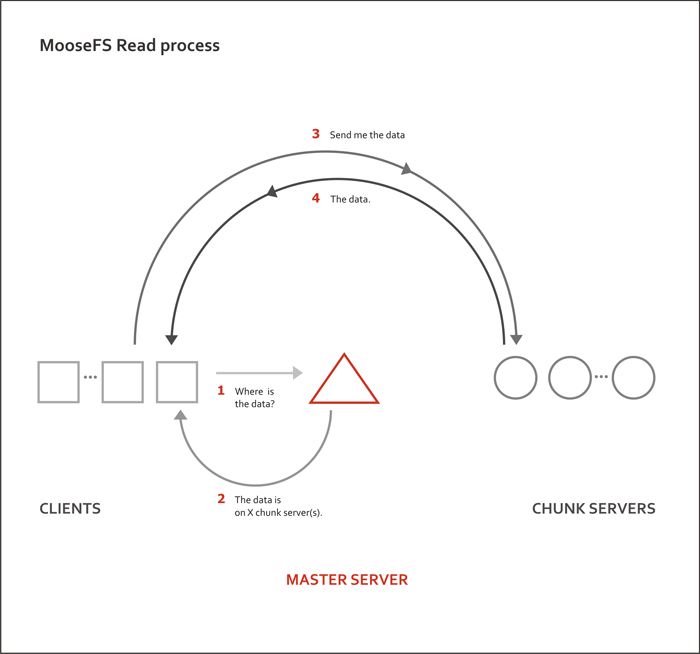
\includegraphics[width=0.8\textwidth]{images/read_mfs.png}\\[1cm]
		\end{center}

		\vfill

		\begin{center}
			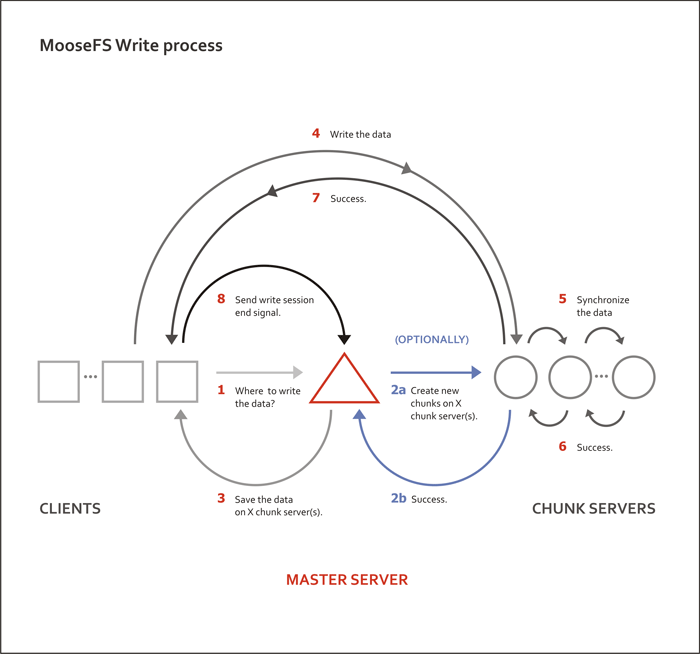
\includegraphics[width=0.8\textwidth]{images/write_mfs.png}\\[1cm]
		\end{center}
		
		Metadata is stored in the memory of the managing server and simultaneously saved to disk (as a periodically updated binary file and immediately updated incremental logs). The main binary file as well as the logs are synchronized to the metaloggers (if present) and to spare master servers in Pro version.
		
		File data is divided into fragments (chunks) with a maximum size of 64MiB each. Each chunk is itself a file on selected disks on data servers (chunkservers).
		
High reliability is achieved by configuring as many different data servers as appropriate to assure the "\code{goal}" value (number of copies to keep) set for the given file.
		
		
		\section{How does the system work}
		All file operations on a client computer that has mounted MooseFS are exactly the same as they would be with other file systems. The operating system's kernel transfers all file operations to the FUSE module, which communicates with the \code{mfsmount} process. The \code{mfsmount} process communicates through the network subsequently with the managing server and data servers (chunk servers). This entire process is fully transparent to the user.\\\\
		
		\code{mfsmount} communicates with the managing server every time an operation on file metadata is required:
		\begin{itemize}
			\item creating files
			\item deleting files
			\item reading directories
			\item reading and changing attributes
			\item changing file sizes
			\item at the start of reading or writing data
			\item on any access to special files on \code{MFSMETA}
		\end{itemize}		

		\bigskip
		\code{mfsmount} uses a direct connection to the data server (chunk server) that stores the relevant chunk of a file. When writing a file, after finishing the write process the managing server receives information from \code{mfsmount} to update a file's length and the last modification time.
		
		Furthermore, data servers (chunk servers) communicate with each other to replicate data in order to achieve the appropriate number of copies of a file on different machines.
		
		\section{Fault tolerance}
		% Add more information
		Administrative commands allow the system administrator to specify the "\code{goal}", or number of copies that should be maintained, on a per-directory or per-file level. Setting the goal to more than one and having more than one data server will provide fault tolerance. When the file data is stored in many copies (on more than one data server), the system is resistant to failures or temporary network outages of a single data server.
		
		This of course does not refer to files with the "\code{goal}" set to 1, in which case the file will only exist on a single data server irrespective of how many data servers are deployed in the system.\\
		
		Exceptionally important files may have their \code{goal} set to a number higher than two, which will allow these files to be resistant to a breakdown of more than one server at the same time.\\
		
		In general the setting for the number of copies available should be one more than the anticipated number of inaccessible or out-of-order servers.\\
		
		In the case where a single data server experiences a failure or disconnection from the network, the files stored within it that had at least two copies, will remain accessible from another data server. The data that is now 'under its goal' will be replicated on another accessible data server to again provide the required number of copies.\\
		
		It should be noted that if the number of available servers is lower than the "\code{goal}" set for a given file, the required number of copies cannot be preserved. Similarly if there are the same number of servers as the currently set goal and if a data server has reached 100\% of its capacity, it will be unable to hold a copy of a file that is now below its goal due to another data server going offline.  In these cases a new data server should be connected to the system as soon as possible in order to maintain the desired number of copies of the file.\\
		
		A new data server can be connected to the system at any time.  The new capacity will immediately become available for use to store new files or to hold replicated copies of files from other data servers.\\
		
		Administrative utilities exist to query the status of the files within the file system to determine if any of the files are currently below their goal (set number of copies). This utility can also be used to alter the goal setting as required.\\
		
		The data fragments stored in the chunks are versioned, so re-connecting a data server with older copy of data (i.e. if it had been offline for a period of time), will not cause the files to become incoherent. The data server will synchronize itself to hold the current versions of the chunks, where the obsolete chunks will be removed and the free space will be reallocated to hold the new chunks.\\
		
		Failures of a client machine (that runs the \code{mfsmount} process) will have no influence on the coherence of the file system or on the other clients' operations. In the worst case scenario the data that has not yet been sent from the failed client computer may be lost.
		
		\section{Platforms}
		MooseFS is available on every Operating System with a working FUSE implementation:
		\begin{itemize}
			\item Linux (Linux 2.6.14 and up have FUSE support included in the official kernel)
			\item FreeBSD
			\item MacOS X
			\item OpenIndiana Hipster
		\end{itemize}
	
		\bigskip	
		The Master Server, Metalogger and Chunkservers can also be run on Windows with Cygwin. Unfortunately without FUSE it won't be possible to mount the filesystem within this operating system.


	\chapter{Moose File System Requirements}

		\section{Network requirements}
		
		MooseFS requires TCP/IP network. The faster the network is, the better is performance. It is recommended to connect all servers to the same switch or at least try to minimize network latencies, because they may have significant impact on performance.
		
		MooseFS requires the following ports to be open (it can be configured in appropriate configuration files):
		
		\begin{itemize}
			\item \code{9419..9421} -- Master Server(s)
			\item \code{9422} -- Chunkservers
			\item \code{9425} -- CGI Server
		\end{itemize}
	
		\section{Requirements for Master Servers}
		As the managing server (master) is a crucial element of MooseFS, it should be installed on a machine which guarantees high stability and access requirements which are adequate for the whole system. It is advisable to use a server with a redundant power supply, ECC memory, and disk array RAID 1 / RAID 5 / RAID 10. The managing server OS has to be POSIX compliant (systems verified so far: Linux, FreeBSD, MacOS X and OpenSolaris).

			\subsection{CPU}
			
			Because Master Server is a single-threaded process, it is recommended to use modern CPU with high clock (e.g. 3.7 GHz) and small number of cores (e.g. 4) -- especially in MooseFS instances which handle a lot of small files.
			
			Additionally, disabling CPU power management in BIOS (or enable mode like "maximum performance") may have positive impact on efficiency.
			
			You can compare CPUs on the following website -- please pay attention to "single-thread points": \code{\url{https://www.cpubenchmark.net/singleThread.html}}.
			

			\subsection{RAM size}
			
			The most important factor in sizing requirements for the Master Server machine is RAM, as the full file system structure is cached in RAM for speed. The Master Server should have approximately 300-350 MiB of RAM allocated to handle 1 million objects (files, directories, pipes, sockets, ...).
			
			\underline{Example}:
			\begin{itemize}
				\item Leader Master RAM usage: \code{20 GiB} (\code{21 017 505 792} Bytes exactly)
				\item "All FS objects" (from MFS CGI): \code{67 552 270}
				\item \code{21 017 505 792 / 67 552 270 = $\sim$311.13} Bytes per one object
			\end{itemize}
			
			\subsection{HDD free space}
		
			The necessary size of HDD depends both on the number of files and chunks used (main metadata file) and on the number of operations made on the files (metadata changelog); for example the space of 20 GiB is enough for storing information for 25 million files and for changelogs to be kept for up to 50 hours.
			
			You can calculate the minimum amount of space we recommend using the following formula:
			\begin{itemize}
				\item \code{RAM} -- amount of RAM
				\item \code{BACK\_LOGS} -- number of metadata change log files, default is 50 (from \code{/etc/mfs/mfsmaster.cfg})
				\item \code{BACK\_META\_KEEP\_PREVIOUS} -- number of previous metadata files to be kept (default is 1) (also from \code{/etc/mfs/mfsmaster.cfg})
			\end{itemize}
			
			\bigskip
			\underline{The formula}: \\
			\code{SPACE = RAM * (BACK\_META\_KEEP\_PREVIOUS + 2) + 1 * (BACK\_LOGS + 1) [GiB]}
			\bigskip
			
			(If default values from \code{/etc/mfs/mfsmaster.cfg} are used, it is \code{RAM * 3 + 51 [GiB]})
			
			The value \code{1} (before multiplying by \code{BACK\_LOGS + 1}) is an estimation of size used by one \code{changelog.[number].mfs} file. On highly loaded MooseFS instance it uses a bit less than 1 GB.
			
			\underline{Example}: \\
			If you have 128 GiB of RAM, using the formula above, you should reserve for \code{/var/lib/mfs}:
			
			128*3 + 51 = 384 + 51 = \textbf{435 GiB minimum}.
		
		\section{Requirements for Metalogger(s)}
		MooseFS metalogger simply gathers metadata backups from the MooseFS Master Server -- so the hardware requirements are not higher than for the Master Server itself; it needs about the same disk space. Similarly to the Master Server -- the OS has to be POSIX compliant (Linux, FreeBSD, Mac OS X, OpenSolaris, etc.).\\
		
		MooseFS Metalogger should have at least the same amount of HDD space (\textbf{especially the free space in \code{/var/lib/mfs}!}) as the main Master Server.
		
		If you would like to use the Metalogger as a Master Server in case of the main Master's failure, the Metalogger machine should have at least the same amount of RAM as the main Master Server.

		\section{Requirements for Chunkservers}
		Chunkservers, like other MooseFS machines have to have POSIX compliant OS.
		
			\subsection{CPU}
			MooseFS Chunkserver is a multi-threaded process, so the best choice is to have a CPU with a number of cores.
			
			\subsection{RAM size}
			MooseFS Chunkserver uses approximately 250 MiB of RAM allocated to handle 1 million chunks.
			
			\underline{Example}:
			\begin{itemize}
				\item Chunkserver RAM usage: \code{661 MiB}
				\item Chunks stored on this Chunkserver (from MFS CGI): \code{3 275 062}
				\item \code{(661 * $2^{20}$) / 3 275 062 = $\sim$211.63} Bytes per one chunk
			\end{itemize}
			
			\subsection{HDD space}
			Chunkserver machines should have appropriate disk space (dedicated exclusively for MooseFS). Typical and recommended usage is to create one partition on each HDD, mount them and enter paths to mounted partitions in \code{/etc/mfs/mfshdd.cfg}.
		
			Minimal configuration should start from several gigabytes of storage space (only disks with more than 256 MB and Chunkservers reporting more than 1 GB of total free space are accessible for new data).

		\section{Requirements for Clients / Mounts}
		\code{mfsmount} requires FUSE to work; FUSE is available on several operating systems: Linux, FreeBSD, OpenSolaris and MacOS X, with the following notes:
		
		\begin{itemize}
			\item In case of Linux a kernel module with API 7.8 or later is required (it can be checked with dmesg command -- after loading kernel module there should be a line fuse init (API version 7.8)). It is available in fuse package 2.6.0 (or later) or in Linux kernel 2.6.20 (or later). Due to some minor bugs, the newer module is recommended (fuse 2.7.2 or Linux 2.6.24, although fuse 2.7.x standalone doesn't contain getattr/write race condition fix).
			\item In case of FreeBSD we recommed using fuse-freebsd\footnote{\url{https://github.com/glk/fuse-freebsd}}, which is a successor to fuse4bsd.
			\item For MacOSX we recommend using OSXFUSE\footnote{\url{http://osxfuse.github.com}}, which is a successor to MacFUSE and has been tested on MacOSX 10.6, 10.7, 10.8, 10.9 and 10.11.
		\end{itemize}




	\chapter{Installing MooseFS 3.0}
	This is a Very Quick Start Guide describing basic MooseFS 3.0 installation in configuration of two Master Servers and three Chunkservers.
	
	Please note that complete installation process is described in "MooseFS Step by Step Tutorial".
	
	For the sake of this document, it's assumed that your machines have following IP addresses:
	\begin{itemize}
		\item Master servers: 192.168.1.1, 192.168.1.2
		\item Chunkservers: 192.168.1.101, 192.168.1.102 and 192.168.1.103
		\item Users' computers (clients): 192.168.2.x
	\end{itemize}

	In this tutorial it is assumed that you have MooseFS 3.0 Pro version. If you use MooseFS 3.0 (non-Pro), please remove '\code{-pro}' from packages names.
	
	\bigskip
	In this tutorial it is also assumed that you have Ubuntu/Debian installed on your machines. If you have another distribution, please use appropriate package manager instead of \code{apt}.	
	
	Note, that most of commands below are preceded by \code{\#} sign, which means, that you have to run such command as \code{root} (\code{\$} sign means normal user). The easiest way to become \code{root} is to run:
		
	\begin{lstlisting}[caption={Becoming \code{root}}]
	$ sudo su -
	\end{lstlisting}
		
		
		\section{Configuring DNS Server}
		Before you start installing MooseFS, you need to have working DNS. It's needed for MooseFS to work properly with several master servers, because DNS can resolve one host name as more than one IP address. \\
		All IPs of machines which will be master servers must be included in DNS configuration file and resolved as "\code{mfsmaster}" (or any other selected name), e.g.:

		\begin{lstlisting}[caption={DNS entries}]
	mfsmaster	IN	A	192.168.1.1		; address of first master server
	mfsmaster	IN	A	192.168.1.2		; address of second master server
		\end{lstlisting}
		
More information about configuring DNS server is included in supplement to "MooseFS Step by Step Tutorial".
		
		\section{Adding repositories}
		Before installing MooseFS you need to add MooseFS Official Supported Repositories to your system.
			\subsection{Ubuntu / Debian}
			First, add the key:
			\begin{lstlisting}[caption={Adding the repo key}]
	# wget -O - http://ppa.moosefs.com/moosefs.key | apt-key add -
			\end{lstlisting}
			
			\bigskip
			Then add the appropriate entry in \code{/etc/apt/sources.list}:
			\begin{itemize}
				\item For Ubuntu 14.04 Trusty: \\
					\code{deb http://ppa.moosefs.com/moosefs-3/apt/ubuntu/trusty trusty main}
				\item For Ubuntu 12.04 Precise: \\
					\code{deb http://ppa.moosefs.com/moosefs-3/apt/ubuntu/precise precise main}
				\item For Ubuntu 10.10 Maverick: \\
					\code{deb http://ppa.moosefs.com/moosefs-3/apt/ubuntu/maverick maverick main}
				\item For Debian 7.0 Wheezy: \\
					\code{deb http://ppa.moosefs.com/moosefs-3/apt/debian/wheezy wheezy main}
				\item For Debian 6.0 Squeeze: \\
					\code{deb http://ppa.moosefs.com/moosefs-3/apt/debian/squeeze squeeze main}
				\item For Debian 5.0 Lenny: \\
					\code{deb http://ppa.moosefs.com/moosefs-3/apt/debian/lenny lenny main}
			\end{itemize}

			\bigskip
			After that do: \\
			\code{\# apt-get update}

			\subsection{RedHat / CentOS (EL7)}
			Red Hat 7 familiy OS use \code{systemd} Linux system and service manager to start processes. To use systemctl command to start MooseFS processes use this steps to add \code{systemd} repository.\\
			
			Add the appropriate key to package manager:
			\begin{lstlisting}[caption={Adding the repo key}]
	# curl "http://ppa.moosefs.com/RPM-GPG-KEY-MooseFS" > /etc/pki/rpm-gpg/RPM-GPG-KEY-MooseFS
			\end{lstlisting}

			Next you need to add the repository entry to yum repo:
			\begin{lstlisting}[caption={Adding MooseFS repo}]
	# curl "http://ppa.moosefs.com/MooseFS-3-el7.repo" > /etc/yum.repos.d/MooseFS.repo
	# yum update
			\end{lstlisting}
			
			\subsection{RedHat / CentOS (EL6)}
			Red Hat 6 family OS use \code{SysV init} runlevel system to start processes. To use service command to start MooseFS processes use this steps to add SysV repository.\\
			Add the appropriate key to package manager:
			\begin{lstlisting}[caption={Adding the repo key}]
	# curl "http://ppa.moosefs.com/RPM-GPG-KEY-MooseFS" > /etc/pki/rpm-gpg/RPM-GPG-KEY-MooseFS
			\end{lstlisting}

			Next you need to add the repository entry to yum repo:
			\begin{lstlisting}[caption={Adding the MooseFS repo}]
	# curl "http://ppa.moosefs.com/MooseFS-3-el6.repo" > /etc/yum.repos.d/MooseFS.repo
	# yum update
			\end{lstlisting}


			\subsection{Apple MacOS X}
			It's possible to run all components of the system on Mac OS X systems, but most common scenario would be to run the client (\code{mfsmount}) that enables Mac OS X users to access resources available in MooseFS infrastructure.
			
			In case of MacOS X -- since there's no default package manager -- we release \code{.pkg} files containing only binaries without any startup scripts, that normally are available in Linux packages.
			
			To install MooseFS on Mac please follow these steps:

			\begin{itemize}
				\item download and install FUSE for Mac OS X package from \\
					\code{http://osxfuse.github.io}
				\item download and install MooseFS packages from \\
					\code{http://ppa.moosefs.com/moosefs-3/osx/}
			\end{itemize}
			
			You should be able to mount MooseFS filesystem in \code{/mnt/mfs} issuing the following command:
			
			\code{\$ sudo mfsmount mfsmount -H mfsmaster.host.name /mnt/mfs}
			
			If you've exported filesystem with additional options like password protection, you should include those options in \code{mfsmount} invocation as in documentation.


		\section{Differences in package names between MooseFS Pro and MooseFS}
		The packages in MooseFS 3.0 Pro are named according to following pattern:
		\begin{itemize}
			\item \code{moosefs-pro-master}
			\item \code{moosefs-pro-metalogger}
			\item \code{moosefs-pro-chunkserver}
			\item \code{moosefs-pro-client}
			\item \code{moosefs-pro-cli}
			\item \code{moosefs-pro-cgi}
			\item \code{moosefs-pro-cgiserv}
			\item \code{moosefs-pro-netdump}
			\item \code{moosefs-pro-supervisor}
		\end{itemize}
		
		\bigskip
		In MooseFS 3.0 (non-Pro) the packages are named according to the following pattern:
		\begin{itemize}
			\item \code{moosefs-master}
			\item \code{moosefs-metalogger}
			\item \code{moosefs-chunkserver}
			\item \code{moosefs-client}
			\item \code{moosefs-cli}
			\item \code{moosefs-cgi}
			\item \code{moosefs-cgiserv}
			\item \code{moosefs-netdump}
		\end{itemize}
		
		\section{MooseFS Master Server(s) installation}
		Install package \code{moosefs-pro-master} by running the following command:
		
		\underline{For Debian OS family}:
		\begin{lstlisting}
	# apt-get install moosefs-pro-master
		\end{lstlisting}
		
		
		\underline{For RedHat OS family}:
		\begin{lstlisting}
	# yum install moosefs-pro-master
		\end{lstlisting}
		
		Sample configuration files will be created in \code{/etc/mfs} with the extension \code{*.sample} (MooseFS 3.0+) or \code{*.dist} (MooseFS 2.0). Use these files as your target configuration files:
		
		\begin{lstlisting}
	# cd /etc/mfs
	# cp mfsmaster.cfg.sample mfsmaster.cfg
	# cp mfsexports.cfg.sample mfsexports.cfg
		\end{lstlisting}

		File \code{mfsexports.cfg} specifies which users' computers can mount the file system and with what privileges. For example, to specify that only machines addressed as \code{192.168.2.x} can use the whole structure of MooseFS resources (\code{/}) in read/write mode, in the first line which is not commented out change the asterisk (\code{*}) to \code{192.168.2.0/24}, so that you'll have:

		\begin{lstlisting}
	192.168.2.0/24		/		rw,alldirs,maproot=0
		\end{lstlisting}
		
		Now, if you use MooseFS Pro, place proper \code{mfslicence.bin} file into \code{/etc/mfs} directory. This file \textbf{must} be available on \textbf{all} Master Servers.
		
		At this point it is possible to run the MooseFS Master Server:
		\begin{lstlisting}
	# mfsmaster start
		\end{lstlisting}
		
		If you use \code{SysV} init script manager, which is by default available in Debian, Ubuntu and RedHat 6 family operating systems, you can also start Master by issuing the following command:

		\begin{lstlisting}
	# service moosefs-pro-master start
		\end{lstlisting}
		
		To start MooseFS Master Server with latest \code{systemd} Linux system and service manager, which is available in RedHat 7 family operating systems, use this command:

		\begin{lstlisting}
	# systemctl start moosefs-pro-master.service
		\end{lstlisting}

		
		You need to repeat these steps on each machine intended for running MooseFS Master Server (in this example -- on \code{192.168.1.1} and \code{192.168.1.2}).
		
		You can also find more detailed description how to add Master Followers in \textbf{MooseFS Upgrade Guide - Chapter 6: Adding master follower(s) server(s) procedure} (Pro only).
	
		\section{MooseFS CGI Monitor, CGI Server and Command Line Interface installation}
		MooseFS CGI Monitor and MooseFS CGISERV can be installed on any machine, but good practice tells that it should be installed on every Master Server.
		
		MooseFS Command Line Interface (CLI) tool allows you to see various information about MooseFS status. The \code{mfscli} with \code{-SIN} option displays basic info similar to the "Info" tab in CGI. To install CGI, CGISERV and CLI, use the following commands.

		\underline{For Debian OS family}:

		\begin{lstlisting}
	# apt-get install moosefs-pro-cgi
	# apt-get install moosefs-pro-cgiserv
	# apt-get install moosefs-pro-cli
		\end{lstlisting}

		Set \code{MFSCGISERV\_ENABLE} variable to \code{true} in file \code{/etc/default/mfs-cgiserv} to configure \code{mfscgiserv} autostart.
	
		\underline{For RedHat OS family}:

		\begin{lstlisting}
	# yum install moosefs-pro-cgi
	# yum install moosefs-pro-cgiserv
	# yum install moosefs-pro-cli
	\end{lstlisting}
	
		
		Run MooseFS CGI Monitor with \code{SysV}:
		\begin{lstlisting}
	# service moosefs-pro-cgiserv start
		\end{lstlisting}
		
		Run MooseFS CGI Monitor with \code{systemd}:
		\begin{lstlisting}
	# systemctl start moosefs-pro-cgiserv.service
		\end{lstlisting}
		MooseFS CGI Monitor website should now be available at \url{http://192.168.1.1:9425} address(for the moment there would be no data about chunk servers).
		
		
		\section{Chunk servers installation}

		\underline{For Debian OS family}:
		\begin{lstlisting}
	# apt-get install moosefs-pro-chunkserver
		\end{lstlisting}
		

		\underline{For RedHat OS family}:
		\begin{lstlisting}
	# yum install moosefs-pro-chunkserver
		\end{lstlisting}

		
		Now you need to prepare basic configuration files for the \code{mfschunkserver}:
		\begin{lstlisting}
	# cd /etc/mfs
	# cp mfschunkserver.cfg.sample mfschunkserver.cfg
	# cp mfshdd.cfg.sample mfshdd.cfg
		\end{lstlisting}
		
		
		In the \code{mfshdd.cfg} file you'll give locations in which you have mounted hard drives/partitions designed for the chunks of the system. It is recommended that they are used exclusively for the MooseFS -- this is necessary to manage the free space properly. For example if you'll use \code{/mnt/mfschunks1} and \code{/mnt/mfschunks2} locations, add these two lines to \code{mfshdd.cfg} file:

		\begin{lstlisting}
	/mnt/mfschunks1
	/mnt/mfschunks2
		\end{lstlisting}


		Before you start chunkserver, make sure that the user \code{mfs} has rights to write in the mounted partitions (which is necessary to create a .lock file):

		\begin{lstlisting}
	# chown -R mfs:mfs /mnt/mfschunks1
	# chown -R mfs:mfs /mnt/mfschunks2
		\end{lstlisting}

		
		At this moment you are ready to start the chunk server:
			
		For \code{SysV} init script system
		\begin{lstlisting}
	# service moosefs-pro-chunkserver start
		\end{lstlisting}
		
		For \code{systemd} Linux system and service manager 
		\begin{lstlisting}
	# systemctl start moosefs-pro-chunkserver.service
		\end{lstlisting}
		
		
		\bigskip
		\bigskip
		You need to repeat these steps on each machine intended for running MooseFS Chunkserver (in this example -- on \code{192.168.1.101}, \code{192.168.1.102} and \code{192.168.1.103}.
		
		Now at \url{http://192.168.1.1:9425} full information about the system is available, including the master server and chunk servers.
		
		
		\section{MooseFS Clients installation}
		MooseFS client uses \code{FUSE} library. During installation process, your operating system also downloads and installs \code{FUSE} library if it is not installed.

		\underline{Debian OS family}:
		\begin{lstlisting}
	# apt-get install moosefs-pro-client
		\end{lstlisting}

		\underline{RedHat OS family}:
		\begin{lstlisting}
	# yum install moosefs-pro-client
		\end{lstlisting}

		Let's assume that you want to mount the MooseFS share in a \code{/mnt/mfs} folder on a client's machine. Issue the following commands:
		\begin{lstlisting}
	# mkdir -p /mnt/mfs
	# mfsmount /mnt/mfs -H mfsmaster
		\end{lstlisting}

		Now after running the \code{df -h | grep mfs} command you should get information similar to this:
		\begin{lstlisting}
	/storage/mfschunks/mfschunks1
		2.0G	69M		1.9G	4%	/mnt/mfschunks1
	/storage/mfschunks/mfschunks2
		2.0G	69M		1.9G	4%	/mnt/mfschunks2
	mfs#mfsmaster:9421
		3.2G	0		3.2G	0%	/mnt/mfs
		\end{lstlisting}
		
		You need to repeat these steps on each machine intended to be MooseFS 3.0 Client (in this example -- on \code{192.168.2.x}.
		
		To enable MooseFS Client automount during boot, first of all check if the \code{fuse} and \code{fuse-libs} packages are installed. If \code{fuse} and \code{fuse-libs} packages are installed, add similar entry to the following one in \code{/etc/fstab}:

		\begin{lstlisting}
	mfsmount    /mnt/mfs    fuse    defaults,mfsmaster=mfsmaster.example.lan,mfsport=9421    0    0 
		\end{lstlisting}
		
		If MooseFS Client has to be mounted on the same machine that MooseFS Master Server runs, please put the following \code{fstab} entry instead of the one listed above:
		
		\begin{lstlisting}
	mfsmount    /mnt/mfs    fuse    defaults,mfsdelayedinit,mfsmaster=mfsmaster.example.lan,mfsport=9421    0    0 
		\end{lstlisting}

		\newpage

		\section{Enabling MooseFS services during OS boot}
		Each operating system has it's own method to manage services start during boot. Below you can find a few examples of enabling MooseFS autostart in supported operating systems.
		
					
		\subsection{RedHat / Centos (EL6)}
		
		\underline{MooseFS Chunkserver}:
		
		To enable MooseFS Chunkserver autostart during OS boot, use \code{chkconfig} command like in example below:
		\begin{lstlisting}
	chkconfig moosefs-chunkserver on
		\end{lstlisting}
		
		\underline{MooseFS Master Server}:
		
		To enable MooseFS Master Server autostart during OS boot, use \code{chkconfig} command like in example below:
		\begin{lstlisting}
	chkconfig moosefs-master on
		\end{lstlisting}
		
		\underline{MooseFS Client}:
		
		To enable MooseFS Client automount during boot, first of all check if the \code{fuse} and \code{fuse-libs} packages are installed:
		\begin{lstlisting}
	# rpm -qa | grep fuse
	fuse-2.8.3-4.el6.x86_64
	fuse-libs-2.8.3-4.el6.x86_64
		\end{lstlisting}
		
		If \code{fuse} and \code{fuse-libs} packages are installed, add similar entry to the following one in \code{/etc/fstab}:

		\begin{lstlisting}
	mfsmount    /mnt/mfs    fuse    defaults,mfsmaster=mfsmaster.example.lan,mfsport=9421    0    0 
		\end{lstlisting}
		
		If MooseFS Client has to be mounted on the same machine that MooseFS Master Server runs, please put the following \code{fstab} entry instead of the one listed above:
		
		\begin{lstlisting}
	mfsmount    /mnt/mfs    fuse    defaults,mfsdelayedinit,mfsmaster=mfsmaster.example.lan,mfsport=9421    0    0 
		\end{lstlisting}



\subsection{RedHat / Centos (EL7)}
		In operating systems with \code{systemd}, use \code{systemctl} command to manage init processes at boot:
		
		\underline{MooseFS Chunkserver}:
		
		To enable MooseFS Chunkserver autostart during OS boot:
		\begin{lstlisting}
	systemctl enable moosefs-chunkserver.service
		\end{lstlisting}
		
		\underline{MooseFS Master Server}:
		
		To enable MooseFS Master Server autostart during OS boot:
		\begin{lstlisting}
	systemctl enable moosefs-master.service
		\end{lstlisting}
		
	
		\underline{MooseFS Client}:
		
		To enable MooseFS Client automount during boot, first of all check if the \code{fuse} and \code{fuse-libs} packages are installed:
		\begin{lstlisting}
	# rpm -qa | grep fuse
	fuse-2.9.2-6.el7.x86_64
	fuse-libs-2.9.2-6.el7.x86_64
		\end{lstlisting}
		
		If \code{fuse} and \code{fuse-libs} packages are installed, add similar entry to the following one in \code{/etc/fstab}:

		\begin{lstlisting}
	mfsmount    /mnt/mfs    fuse    mfsmaster=mfsmaster.example.lan,mfsport=9421    0    0 
		\end{lstlisting}

		If MooseFS Client has to be mounted on the same machine that MooseFS Master Server runs, please put the following \code{fstab} entry instead of the one listed above:
		
		\begin{lstlisting}
	mfsmount    /mnt/mfs    fuse    defaults,mfsdelayedinit,mfsmaster=mfsmaster.example.lan,mfsport=9421    0    0 
		\end{lstlisting}
		

		\subsection{Debian / Ubuntu}
		This method works in Debian 6, Debian 7, Ubuntu 12, Ubuntu 14.
		
		\underline{MooseFS Chunkserver}:
		
		To enable MooseFS Chunkserver autostart during OS boot, find \code{/etc/default/moosefs-chunkserver} file and change \code{MFSCHUNKSERVER\_ENBLE} variable to \code{true}:
		\begin{lstlisting}
	MFSCHUNKSERVER_ENABLE=true
		\end{lstlisting}
		
		\underline{MooseFS Master}:
		
		To enable MooseFS Master Server autostart during OS boot, edit \code{/etc/default/moosefs-master} file and change \code{MFSMASTER\_ENBLE} variable to \code{true}:
		\begin{lstlisting}
	MFSMASTER_ENABLE=true
		\end{lstlisting}

		\underline{MooseFS Client}:
			
		To enable MooseFS Client automount during boot, first of all check if the \code{fuse} and \code{fuse-libs} packages are installed. If \code{fuse} and \code{fuse-libs} packages are installed, add similar entry to the following one in \code{/etc/fstab}:

		\begin{lstlisting}
	mfsmount    /mnt/mfs    fuse    mfsmaster=mfsmaster.example.lan,mfsport=9421    0    0 
		\end{lstlisting}

		If MooseFS Client has to be mounted on the same machine that MooseFS Master Server runs, please put the following \code{fstab} entry instead of the one listed above:
		
		\begin{lstlisting}
	mfsmount    /mnt/mfs    fuse    defaults,mfsdelayedinit,mfsmaster=mfsmaster.example.lan,mfsport=9421    0    0 
		\end{lstlisting}


		
				
		\subsection{FreeBSD}

		\underline{MooseFS Chunkserver}:
		
		To enable MooseFS Chunkserver autostart during OS boot, add an entry to \code{/etc/rc.conf}:
		\begin{lstlisting}
	mfschunkserver_enable="YES"
		\end{lstlisting}
		
		\underline{MooseFS Master}:
		
		To enable MooseFS Chunkserver autostart during OS boot, add entry to \code{/etc/rc.conf}:
		\begin{lstlisting}
	mfsmaster_enable="YES"
		\end{lstlisting}

		\underline{MooseFS Client}:
		
		To enable MooseFS Client automount during boot add the following entry in \code{/boot/loader.conf} to let FreeBSD load \code{fuse} module during boot:
		\begin{lstlisting}
	fuse_load="YES"
		\end{lstlisting}
		
		And add the entry in \code{/etc/fstab}:
		\begin{lstlisting}
	mfsmount_magic /mnt/mfs moosefs rw,mfsmaster=mfsmaster,mountprog=/usr/local/bin/mfsmount,late 0 0 
		\end{lstlisting}

		
		\newpage
	
		\section{Basic MooseFS use}
		Create \code{folder1} in \code{/mnt/mfs}, in which you store files in one copy (setting \code{goal=1}):
		\begin{lstlisting}
	mkdir -p /mnt/mfs/folder1
		\end{lstlisting}

and \code{folder2}, in which you store files in two copies (setting \code{goal=2}):
		\begin{lstlisting}
	mkdir -p /mnt/mfs/folder2
		\end{lstlisting}


		The number of copies for the folder is set with the \code{mfssetgoal -r} command:
		\begin{lstlisting}
	# mfssetgoal -r 1 /mnt/mfs/folder1
	/mnt/mfs/folder1:
	inodes with goal changed:				0
	inodes with goal not changed:			1
	inodes with permission denied:			0

	# mfssetgoal -r 2 /mnt/mfs/folder2
	/mnt/mfs/folder2:
	inodes with goal changed:				0
	inodes with goal not changed:			1
	inodes with permission denied:			0
		\end{lstlisting}

	
		\section{Stopping MooseFS}
		In order to safely stop the MooseFS cluster you have to perform the following steps:
		\begin{itemize}
			\item Unmount the file system on all machines using umount command (in our example it would be: \code{umount /mnt/mfs})
			\item Stop the Chunk Servers processes:\\
				For \code{SysV}: \code{service moosefs-pro-chunkserver stop}\\
				For \code{systemd}: \code{systemctl stop moosefs-pro-chunkserver.service}
				 
			\item Stop the Master Server processes (starting from the FOLLOWER, you shuould stop the LEADER Master Server as the last one):\\
				For \code{SysV}: \code{service moosefs-pro-master stop}\\
				For \code{systemd}: \code{systemctl stop moosefs-pro-master.service}			
			
			\item Stop the Metalogger process:\\
				For \code{SysV}: \code{service moosefs-pro-metalogger stop}\\
				For \code{systemd}: \code{systemctl stop moosefs-pro-metalogger.service}		
		\end{itemize}	
	
	
	\chapter{Storage Classes}
		\section{Introduction to Storage Classes functionality in MooseFS 3.0}
			
			\subsection{What is a Storage Class?}
			Since MooseFS 3.0 goal has been extended to Storage Class. Storage Classes allow you to specify on which Chunkservers copies of files should be stored. Storage Classes are defined using label expressions.
			
			 To maintain compatibility with standard goal semantics, there are predefined Storage Classes from 1 to 9 that, unless changed behave like goals from MooseFS 2.0 or 1.6 (see \textbf{Subsection "\nameref{section:predefined-storage-classes}" of Section \ref{section:moosefs-storage-class-administration-tool}: \nameref{section:moosefs-storage-class-administration-tool}} of this manual or \code{man mfsscadmin}). Goal tools simply work only on these classes.	
			
			\subsection{What are labels?}
			Labels are letters (A-Z -- 26 letters) that can be assigned to Chunkservers. Each chunkserver can have multiple (up to 26) labels.
			
			Labels expression is a set of subexpressions separated by commas, each subexpression specifies the storage schema of one copy of a file. Subexpression can be: an asterisk or a label schema.
			
			Label schema can be one label or an expression with sums, multiplications and brackets. Sum means a file can be stored on any chunkserver matching any element of the sum (logical or). Multiplication means a file can be stored only on a chunkserver matching all elements (logical and).  Asterisk means any chunkserver.
			
			Identical subexpressions can be shortened by adding a number in front of one instead of repeating it a number of times.
			
			For more information about labels expressions, refer to \textbf{Subsection "\nameref{section:labels-expressions}" of Section \ref{section:moosefs-storage-class-administration-tool}: \nameref{section:moosefs-storage-class-administration-tool}} of this manual.
	
	
			
		\section{How to use Storage Classes?}
			\subsection{Machines configuration}
			In this example we have MooseFS 3.0 installed on 11 machines:
			\begin{itemize}
				\item \code{ts02}, \code{ts03} -- Master Servers
				\item \code{ts04..ts12} -- Chunkservers
			\end{itemize}
			\bigskip
			
			Assumption:
			\begin{itemize}
			\item On the MooseFS instance there is some initial data stored with goal \code{2} (Storage Class \code{2}).
			\end{itemize}
			
			\subsection{Example of MooseFS installation without Storage Classes}
			To run MooseFS without any user-defined Storage Classes, you don't have to make any changes in configuration. Just install MooseFS with default configuration. The process is described in "\textbf{MooseFS Step by Step Tutorial}".
			
			The picture below shows the discussed installation:
			
			\bigskip
			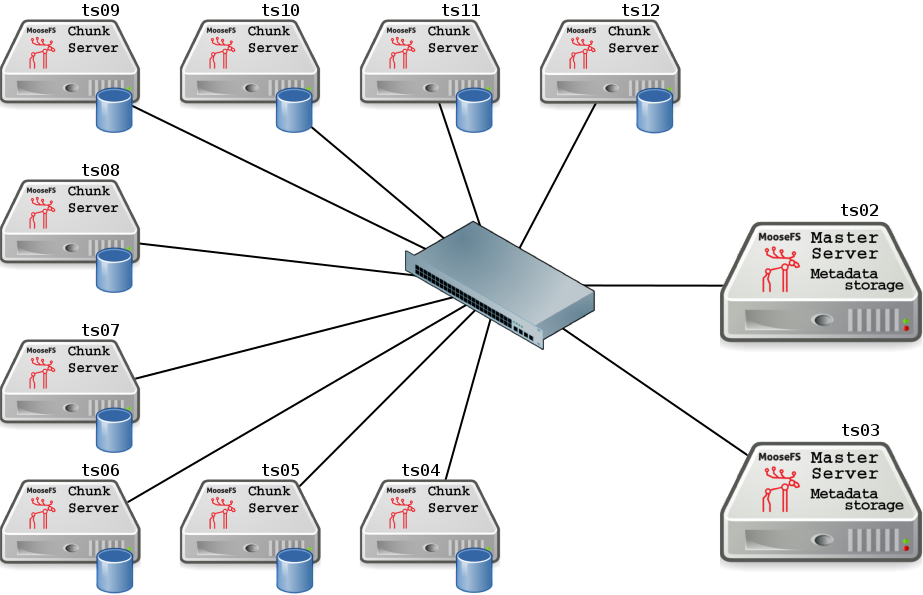
\includegraphics[scale=0.5]{images/diagram_without_labels.png}
	
			\pagebreak
			
			If labels on Chunkservers are not set up, the system is balanced like MooseFS 2.0. The image below presents system balance at this point:
			
			\bigskip
			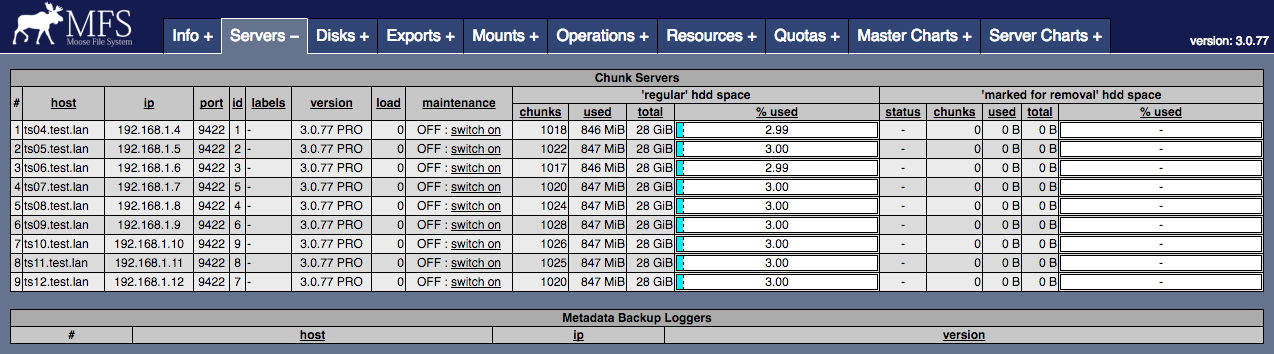
\includegraphics[width=1.0\textwidth]{images/cgi_nolabels.png}
			
			\subsection{Labelling Chunkservers}
			To add labels to the system, i.e. assign them to Chunkservers, you need to edit their configuration files (\code{/etc/mfs/mfschunkserver.cfg}). Open the file, uncomment the following line and after the equation character type labels you want to set on specific Chunkserver. For example to set label \code{A} on Chunkservers ts04, ts05, ts06 and ts07, their configuration should look like this:
			
			\begin{lstlisting}
	[...]
	
	# labels string (default is empty - no labels)
	LABELS = A
	
	[...]
			\end{lstlisting}
			
			
			The next step is to "inform" the Chunkserver, that the Configuration file has changed. Issue the command:
			\begin{lstlisting}
	root@chunkserver:~# service moosefs-pro-chunkserver reload
			\end{lstlisting}
			
			or:
			\begin{lstlisting}
	root@chunkserver:~# mfschunkserver reload
			\end{lstlisting}
			
	
			Similarly set label \code{B} for Chunkservers ts08, ts09, ts10, ts11, ts12.		
			
			After this step in CGI monitor you can observe, that Chunkservers ts04..ts07 have label \code{A} and Chunkservers ts08..ts12 -- label \code{B}:
			
			\bigskip
			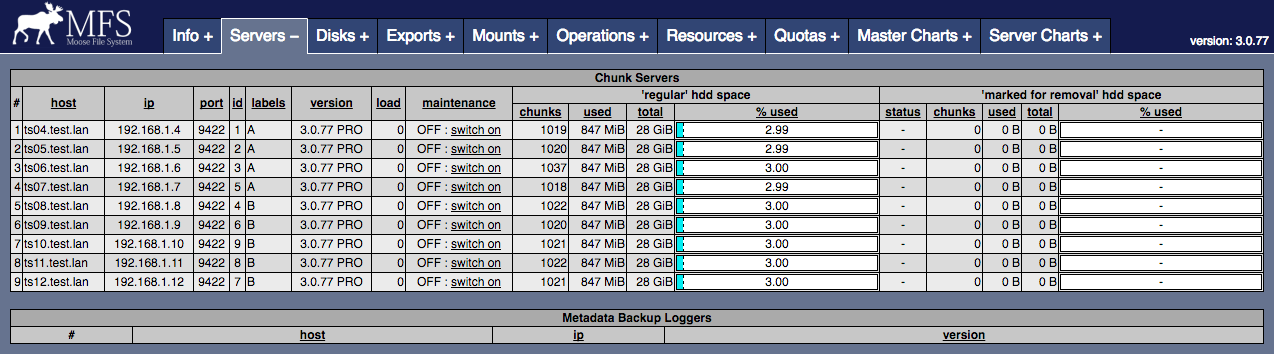
\includegraphics[width=1.0\textwidth]{images/cgi_labelsAB.png}
	
			\bigskip
					
			\underline{Notice}: If you want to set more than one label for a Chunkserver, just enter appropriate labels in configuration file (\code{/etc/mfs/mfschunkserver.cfg}). MooseFS supports schemes listed below, so you can choose the one, which fits for you the best, e.g.:
			
			\bigskip
			
			\begin{lstlisting}
	[...]
	# labels string (default is empty - no labels)
	LABELS = XYZ
	[...]
			\end{lstlisting}
			
			or:
			
			\begin{lstlisting}
	[...]
	# labels string (default is empty - no labels)
	LABELS = X, Y, Z
	[...]
			\end{lstlisting}
			
			or:
			
			\begin{lstlisting}
	[...]
	# labels string (default is empty - no labels)
	LABELS = X Y Z
	[...]
			\end{lstlisting}
			
			\bigskip
			
			The picture below presents current system configuration:			
			\bigskip
	
			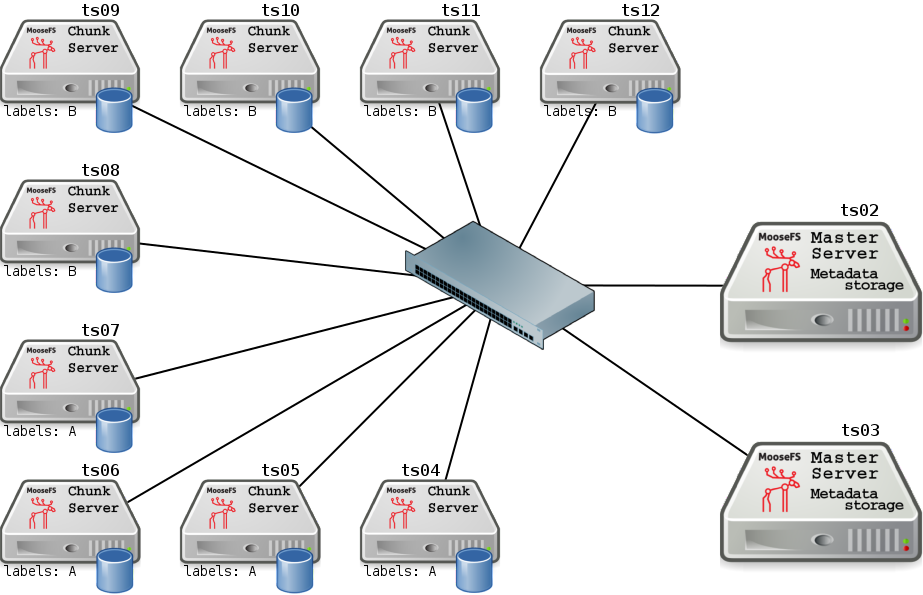
\includegraphics[scale=0.5]{images/diagram_with_labels.png}
	
			\pagebreak
			
			\subsection{Creating Storage Classes}
			
			In order to create a Storage Class on MooseFS, use the \code{mfsscadmin} tool. Below you can find a simple example, you can read a full description of \code{mfsscadmin} usage in \textbf{Chapter \ref{chapter:storage-classes-tools}:  \nameref{chapter:storage-classes-tools}} or in \code{man mfsscadmin}.
			
			Let's create a storage class named \code{sclass1}:
			
			First of all, mount MooseFS:
			
			\begin{lstlisting}[caption={Mounting MooseFS (Linux only)}]
	root@client:~# mount -t moosefs mfsmaster.test.lan: /mnt/mfs
	mfsmaster 192.168.1.2 - found leader: 192.168.1.3
	mfsmaster accepted connection with parameters: read-write,restricted_ip,admin ; root mapped to root:root
	root@client:~#
			\end{lstlisting}
			
			or
			
			\begin{lstlisting}[caption={Mounting MooseFS (universal)}]
	root@client:~# mfsmount -H mfsmaster.test.lan /mnt/mfs
	mfsmaster 192.168.1.2 - found leader: 192.168.1.3
	mfsmaster accepted connection with parameters: read-write,restricted_ip,admin ; root mapped to root:root
	root@client:~#
			\end{lstlisting}
			
			Then, navigate to mounted file system:
			\begin{lstlisting}
	root@client:~# cd /mnt/mfs
	root@client:/mnt/mfs#
			\end{lstlisting}
			
			Let's assume, you want to have your files stored in 2 copies on Chunkservers labelled as \code{A}. Create a Storage Class with appropriate definition:
			
			\begin{lstlisting}
	root@client:/mnt/mfs# mfsscadmin create 2A sclass1
	create ; 0
	storage class make sclass1: ok
	root@client:/mnt/mfs#
			\end{lstlisting}
			
			It means that every file with \code{sclass1} assigned will be stored in two copies: one will be kept on Chunkserver with label A, another one -- on another Chunkserver with label A.
			
			Similarly, create a Storage Class \code{sclass2}, which keep 2 copies on Chunkservers labelled as \code{B}:
			
			\begin{lstlisting}
	root@client:/mnt/mfs# mfsscadmin create 2B sclass2
	create ; 0
	storage class make sclass2: ok
	root@client:/mnt/mfs#
			\end{lstlisting}
			
			\underline{Notice}: You don't have to navigate to mounted file system to create a Storage Class -- it is also possible to do it from any location. In such case just let \code{mfsscadmin} tool know, where MooseFS is mounted (in first parameter), e.g.:
			
			\begin{lstlisting}
	root@client:~# mfsscadmin /mnt/mfs create 2B sclass2
			\end{lstlisting}
			
			It applies to all Storage Classes tools.
			
			\pagebreak
			
			\subsection{Listing Storage Classes}
			
			Now, let's check, if the classes has been properly created and are available to use:
			
			\begin{lstlisting}
	root@client:/mnt/mfs# mfsscadmin list
	list ; 1
	1
	2
	3
	4
	5
	6
	7
	8
	9
	sclass1
	sclass2
	root@client:/mnt/mfs#
			\end{lstlisting}
			
			You can also see more detailed view by issuing the command with \code{-l} switch:
			
			\begin{lstlisting}
	root@client:/mnt/mfs# mfsscadmin list -l
	list ; 1
	[...]
	sclass1 : 2 ; admin_only: NO ; create_mode: STD ; create_labels: [A] , [A] ; keep_labels: [A] , [A]
	sclass2 : 2 ; admin_only: NO ; create_mode: STD ; create_labels: [B] , [B] ; keep_labels: [B] , [B]
	root@client:/mnt/mfs#
			\end{lstlisting}
	
			\subsection{Assigning Storage Class to files / directories}
	
			There are several tools to manage Storage Classes assignment to files, directories etc.: \code{mfsgetsclass}, \code{mfssetsclass}, \code{mfscopysclass}, \code{mfsxchgsclass}, \code{mfslistsclass}. You can find out more about them in \textbf{Section \ref{section:moosefs-storage-class-management-tools}:  \nameref{section:moosefs-storage-class-management-tools}} or by issuing \code{man mfssclass}.
			
			Now it's time to store some data on this MooseFS instance. Create two directories, let's say \code{dataX} and \code{dataY}.
	
			\begin{lstlisting}
	root@client:~# cd /mnt/mfs
	root@client:/mnt/mfs# mkdir dataX
	root@client:/mnt/mfs# mkdir dataY
	root@client:/mnt/mfs#
			\end{lstlisting}
			
			Next, assign Storage class \code{sclass1} to \code{/mnt/mfs/dataX}:
			\begin{lstlisting}
	root@client:/mnt/mfs# mfssetsclass sclass1 dataX
	dataX: storage class: 'sclass1'
	root@client:/mnt/mfs#
			\end{lstlisting}
			
			It means that this directory, its subdirectories, files and so on will be stored according to \code{sclass1} policy.
			
			Similarly, assign Storage class \code{sclass2} to \code{/mnt/mfs/dataY}:
					
			\begin{lstlisting}
	root@client:/mnt/mfs# mfssetsclass sclass2 dataY
	dataY: storage class: 'sclass2'
	root@client:/mnt/mfs#
			\end{lstlisting}
			
			It means that this directory, its subdirectories, files and so on will be stored according to \code{sclass2} policy.
			
			
	
			
			For more information about assigning Storage Classes to files, refer to \textbf{Section \ref{section:moosefs-storage-class-management-tools}:  \nameref{section:moosefs-storage-class-management-tools}}.
			
			Now on MooseFS Monitor ("Resources" tab) you can observe, that goal is set and it can be fulfilled.
			
			\bigskip
			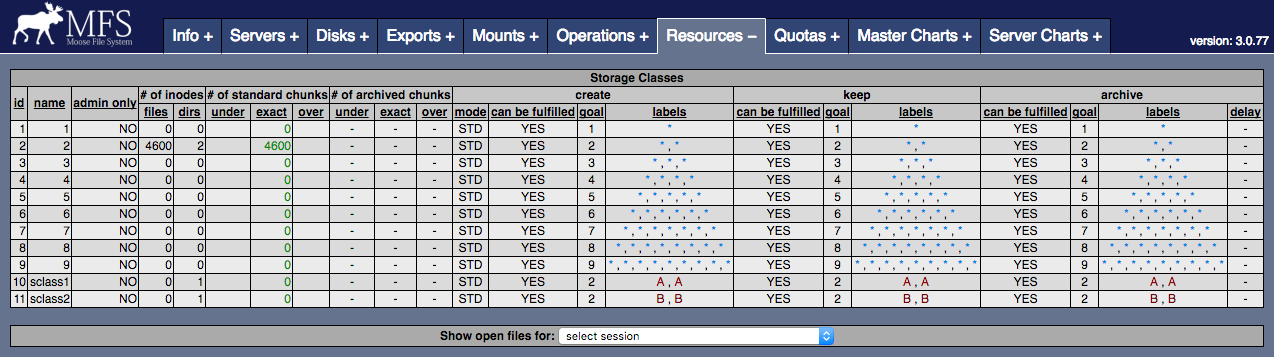
\includegraphics[width=1.0\textwidth]{images/cgi_resources1.png}
				
				\subsubsection{Creating files}
				In this step you will create some files in previously created directories (\code{labelA} and \code{labelB}) to fill MooseFS instance with data. This operation may take some time. Issue the following commands:
				
				\begin{lstlisting}
	root@client:/mnt/mfs# cd dataX
	root@client:/mnt/mfs/dataX# for i in `seq 1 35`; do dd if=/dev/urandom of=dd1G_$i.bin bs=1M count=1024; done
	[...]
	root@client:/mnt/mfs/dataX# cd ../dataY
	root@client:/mnt/mfs/dataY# for i in `seq 1 10`; do dd if=/dev/urandom of=dd1G_$i.bin bs=1M count=1024; done
	[...]
	root@client:/mnt/mfs/dataY#
				\end{lstlisting}
				
				\underline{Notice}: These commands create approx. 90 GiB (45 GiB multiplied by goal 2) of data -- 35 GiB in \code{dataX} directory (RAW size: 70 GiB) and 10 GiB in \code{dataY} directory (RAW size: 20 GiB), so adjust them for your testing purposes.
	
				\subsubsection{Filesystem balance with Storage Classes applied}
				Now you can observe, that filesystem is balanced according to Storage Classes policy: Chunkservers with label A store the data data with goal \code{2A} applied, similarly -- Chunkservers with label B store the data with goal \code{2B}:
				
				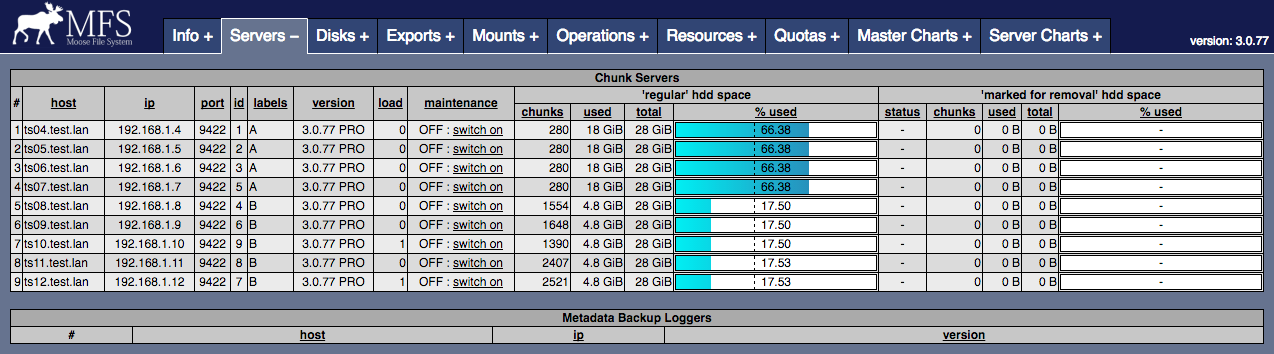
\includegraphics[width=1.0\textwidth]{images/cgi_labelsAB_data.png}
				
				\textbf{Notice, that the system looks "unbalanced", but it is, in fact, balanced as much, as the requirements of Storage Classes allow it to be.}
				
				Also in tab "Resources" number of inodes has changed:
				
				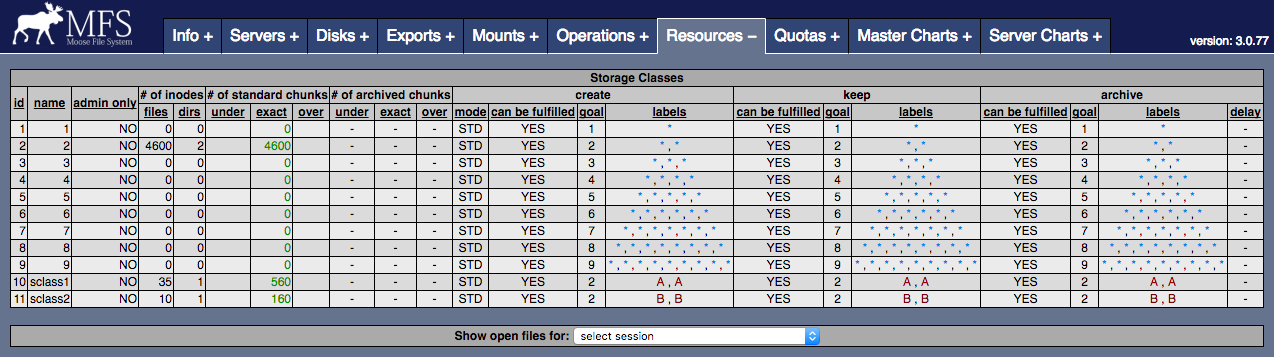
\includegraphics[width=1.0\textwidth]{images/cgi_resources2.png}
			
			\subsection{Creation, keep, archive labels}
			In MooseFS 3.0 a possibility to "plan" changing labels has been added.
			
			Now you can "tell" MooseFS (crate appropriate Storage Class), what label expression it should use for file(s) while creating it (them), to what label expression change it after the creation and to what label expression change it after a specific time since last modification.
			
			You can define it while creating a Storage Class by \code{mfsscadmin} tool.
			
				\subsubsection{Synopsis}
				\code{mfsscadmin [/MOUNTPOINT] create|make [-a admin\_only] [-m creation\_mode]} \\ \code{[-C CREATION\_LABELS] -K KEEP\_LABELS [-A ARCH\_LABELS -d ARCH\_DELAY] SCLASS\_NAME...}
			
				\subsubsection{Creation labels}
				"Creation labels" (\code{-C CREATION\_LABELS}) -- optional parameter, that tells the system to which Chunkservers, defined by the \code{CREATION\_LABELS} expression, the chunk should be first written just after creation; if this parameter is not provided for a class, the \code{KEEP\_LABELS} Chunkservers will be used.
			
			
				\subsubsection{Keep labels}
				"Keep labels" (\code{-K KEEP\_LABELS}) -- mandatory parameter (assumed in the second, abbreviated version of the command), that tells the system on which Chunkservers, defined by the \code{KEEP\_LABELS} expression, the chunk(s) should be kept always, except for special conditions like creating and archiving, if defined.
			
				\subsubsection{Archive labels}
				"Archive labels" (\code{-A ARCH\_LABELS -d ARCH\_DELAY}) -- optional parameter, that tells the system on which Chunkservers, defined by the \code{ARCH\_LABELS} expression, the chunk(s) should be kept for archiving purposes; the system starts to treat a chunk as archive, when the last \underline{modification time} (\code{mtime}) of the file it belongs to is older than the number of days specified with \code{-d} parameter.
				
				\subsubsection{How to set it?}
				For more information about the command to issue, refer to \textbf{Section \ref{section:moosefs-storage-class-administration-tool}:  \nameref{section:moosefs-storage-class-administration-tool}} or issue \code{man mfsscadmin}.
				
			\subsection{Chunkserver states}
			Chunkserver can work in 3 states: \code{normal}, \code{overloaded} and (since MooseFS 3.0.62) \code{internal rebalance}:
			
			\begin{itemize}
				\item \code{Normal} state is a standard state. In "Servers" CGI tab you can see load as a normal number, e.g.: \code{7}.
				\item \code{Internal rebalance} state is a special Chunkserver state. It is activated when e.g. you add a new, empty HDD to a Chunkserver. Then Chunkserver enters this special mode and rebalances chunks between all HDDs to make all HDDs utilization as close to equal as possible. In "Servers" CGI tab you can see load as number in round brackets, e.g.: \code{(7)}.
				\item \code{Overloaded} is a special, \textbf{temporary} Chunkserver state. It is activated when Chunkserver load is high and Chunkserver is not able to perform more operations at the moment. In such case, Chunkserver sends an information to Master Server that it is overloaded. If the load lowers to the normal level, Chunkserver sends an information to Master Server, that it is not overloaded any more. In "Servers" CGI tab you can see load as a number in square brackets, e.g.: \code{[77]}.
			\end{itemize}
	

			\subsection{Chunk creation modes}
			While you store your data on labelled Chunkservers, a situation may occur that there is no more space on appropriate Chunkservers or they are overloaded.
			
			To decide what MooseFS should do when free space ends or when Chunkserver you want to store data to is overloaded, you need to use creating chunks modes.
			
			You can define these modes for each file, directory, it's subdirectories and so on, because they can be set (or modified) when you set the goal for your data.
			
			There are three modes:
			
			\begin{itemize}
				\item \code{loose} mode (\code{-m L} flag to \code{mfsscadmin}) -- in this mode the system will use other servers in case of overloaded servers or no space on servers and will replicate data to correct servers when it becomes possible.
				\item \code{default} mode (no flag or \code{-m D} flag to \code{mfsscadmin}) -- in case of overloaded servers system will wait for them, but in case of no space available will use other servers and will replicate data to correct servers when it becomes possible.
				\item \code{strict} mode (\code{-m S} flag to \code{mfsscadmin}) -- in this mode the system will return error (\code{ENOSPC}) in case of no space available on servers marked with labels specified for chunk creation. It will still wait for overloaded servers.
			\end{itemize}
			
			\bigskip
			A table below presents MooseFS behavior for these modes:
			\bigskip
			
			\begin{tabular}{r|c|c}
									& \textbf{Chunkserver is full}		& \textbf{Chunkserver is overloaded} \\
				\hline
				\textbf{Loose}		& use servers with other labels		& use servers with other labels \\
				\hline
				\textbf{Default}		& use servers with other labels 		& wait for available Chunkserver \\
				\hline
				\textbf{Strict}		& no write (returns \code{ENOSPC})	& wait for available Chunkserver \\
			\end{tabular}
			\bigskip
			
			You can observe current states in Resources CGI tab.
	
			\subsection{Preferred labels during read/write (in \code{mfsmount})}
			It is possible to specify preferred labels for choosing Chunkservers during read and write operations at the MooseFS Client (\code{mfsmount}) side:
			
			\begin{lstlisting}
			-o mfspreflabels=LABELEXPR
	              specify preferred labels for choosing Chunkservers during I/O
			\end{lstlisting}
			
			You can set different preferred labels for each mountpoint.
			
			Preferred labels in MooseFS Client are a list (up to 9) of labels expressions, e.g. $E_{1}$, $E_{2}$, $E_{3}$.
			
			While a client performs a read operation, Master Server returns a list of chunks' locations (in random order) in the following form (CS means Chunkserver): $CS_{a}$, $CS_{b}$, $CS_{c}$, ...
	
			Each of $CS_{x}$ entry contains a list of labels assigned to specific Chunkserver.
			
			Priority of each $CS_{x}$ is calculated as the minimum $y$ value, where labels from $CS_{x}$ match expression $E_{y}$. If no expression matches, the priority is set as a number of expressions $+1$.
	
			The lowest number means the highest priority.
	
			Then, the list of Chunkservers is sorted by priorities. The first Chunkserver from the list (which has the highest priority / the lowest number) is used while reading.
			
			If more than one Chunkserver has the same priority, Client picks the one that got the least number of operations from this Client so far.
			
			If a specific chunk read ends with an error, Client can use a chunk copy with lower priority (greater number).
	
			In case of writing, the list of Chunkservers is sorted similarly and data is written to Chunkserver with the highest priority. The difference is, if more that one Chunkserver has the same priority, the order form Master Server is used.
			
			If no \code{mfspreflabels} is set, the order of list from MooseFS Master is used with no further modifications.
			
			
			
		\section{Storage Classes tools}
			\label{chapter:storage-classes-tools}
	
			\subsection{MooseFS Storage Class administration tool -- \code{mfsscadmin}}
				\label{section:moosefs-storage-class-administration-tool}
				
				\subsubsection{Synopsis}
				
					\begin{itemize}
						\item \code{mfsscadmin [/MOUNTPOINT] create|make [-a admin\_only] [-m creation\_mode] [-C CREATION\_LABELS] -K KEEP\_LABELS [-A ARCH\_LABELS -d ARCH\_DELAY] SCLASS\_NAME...}
						\item \code{mfsscadmin [/MOUNTPOINT] create|make [-a admin\_only] [-m creation\_mode] LABELS SCLASS\_NAME...}
						\item \code{mfsscadmin [/MOUNTPOINT] change|modify [-f] [-a admin\_only] [-m creation\_mode] [-C CREATION\_LABELS] [-K KEEP\_LABELS] [-A ARCH\_LABELS] [-d ARCH\_DELAY] SCLASS\_NAME...}
						\item \code{mfsscadmin [/MOUNTPOINT] delete|remove SCLASS\_NAME...}
						\item \code{mfsscadmin [/MOUNTPOINT] copy|duplicate SRC\_SCLASS\_NAME DST\_SCLASS\_NAME...}
						\item \code{mfsscadmin [/MOUNTPOINT] rename SRC\_SCLASS\_NAME DST\_SCLASS\_NAME}
						\item \code{mfsscadmin [/MOUNTPOINT] list [-l]}
					\end{itemize}
					
				\subsubsection{Description}
					
					\code{mfsscadmin} is a tool for defining storage classes, which can be later applied to MooseFS objects with mfssetsclass, mfsgetsclass etc.
					
					Storage class is a set of labels expressions and options that indicate, on which chunkservers the files in this class should be written and later kept.
				
				\subsubsection{Commands}
					
					\begin{itemize}
						\item \code{create|make} creates a new storage class with given options, described below and names it \code{SCLASS\_NAME}; there can be more than one name provided, multiple storage classes with the same definition will be created then
					
						\item \code{change|modify} -- changes the given options in a class or classes indicated by \code{SCLASS\_NAME} paremeter(s)
					
						\item \code{delete|remove} -- removes the class or classes indicated by \code{SCLASS\_NAME} paremeter(s); if any of the classes is not empty (i.e. it is still used by some MooseFS objects), it will not be removed and the tool will return an error and an error message will be printed; empty classes will be removed in any case
					
						\item \code{copy|duplicate} -- copies class indicated by \code{SRC\_SCLASS\_NAME} under a new name provided with \code{DST\_SCLASS\_NAME}
						
						\item \code{rename} -- changes the name of a class from \code{SRC\_SCLASS\_NAME} to \code{DST\_SCLASS\_NAME}
						
						\item \code{list} -- lists all the classes
					\end{itemize}
				
				\subsubsection{Options}
					
					\begin{itemize}
		
						\item \code{-C} -- optional parameter, that tells the system to which chunkservers, defined by the \code{CREATION\_LABELS} expression, the chunk should be first written just after creation; if this parameter is not provided for a class, the \code{KEEP\_LABELS} chunkservers will be used
				
						\item \code{-K} -- mandatory parameter (assumed in the second, abbreviated version of the command), that tells the system on which chunkservers, defined by the \code{KEEP\_LABELS} expression, the chunk(s) should be kept always, except for special conditions like creating and archiving, if defined
				
						\item \code{-A} -- optional parameter, that tells the system on which chunkservers, defined by the \code{ARCH\_LABELS} expression, the chunk(s) should be kept for archiving purposes; the system starts to treat a chunk as archive, when the last modification time of the file it belongs to is older than  the  number  of days specified with \code{-d} option
				
						\item \code{-d} -- optional parameter that \textbf{must} be defined when \code{-A} is defined, \code{ARCH\_DELAY} parameter defines after how many days from last modification time a file (and its chunks) are treated as archive
				
						\item \code{-a} -- can be either 1 or 0 and indicates if the storage class is available to everyone (0) or admin only (1)
				
						\item \code{-f} -- force the changes on a predefined storage class (see below), use with caution!
				
						\item \code{-m} -- is described below in "Creation modes" section
				
						\item \code{-l} -- list also definitions, not only the names of existing storage classes			
					
					\end{itemize}
				
				\subsubsection{Labels expressions}
					\label{section:labels-expressions}
					Labels are letters (A-Z -- 26 letters) that can be assigned to chunkservers. Each chunkserver can have multiple (up to 26) labels. Labels are defined in \code{mfschunkserver.cfg} file, for more information refer to the appropriate manpage.
				
					Labels expression is a set of subexpressions separated by commas, each subexpression specifies the storage schema of one copy of a file. Subexpression can be: an asterisk or a label schema.
					
					Label schema can be one label or an expression with sums, multiplications and brackets. Sum means a file can be stored on any chunkserver matching any element of the sum (logical or).
					
					Multiplication means a file can be stored only on a chunkserver matching all elements (logical and).  Asterisk means any chunkserver. Identical subexpressions can be shortened by adding a  number  in  front  of  one	instead of repeating it a number of times.
		
					\bigskip		
				
					\underline{Examples of labels expressions}:
				
					\begin{itemize}
						\item \code{A,B} -- files will have two copies, one copy will be stored on chunkserver(s) with label \code{A}, the other on chunkserver(s) with label \code{B}
				
						\item \code{A,*} -- files will have two copies, one copy will be stored on chunkserver(s) with label \code{A}, the other on any chunkserver(s)
				
						\item \code{*,*} -- files will have two copies, stored on any chunkservers (different for each copy)
					
						\item \code{AB,C+D} -- files will have two copies, one copy will be stored on any chunkserver(s) that has both labels \code{A} and \code{B} (\textbf{multiplication of labels}), the other on any chunkserver(s) that has either the \code{C} label or the \code{D} label (\textbf{sum of labels})
				
						\item \code{A,B[X+Y],C[X+Y]} -- files will have three copies, one copy will be stored on any chunkserver(s) with A label, the second on any chunkserver(s) that has the \code{B} label and either \code{X} or \code{Y} label, the third on any chunkserver(s), that has the \code{C} label and either \code{X} or \code{Y} label
				
						\item \code{A,A} expression is equivalent to \code{2A} expression
				
						\item \code{A,BC,BC,BC} expression is equivalent to \code{A,3BC} expression
				
						\item \code{*,*} expression is equivalent to \code{2*} expression is equivalent to \code{2} expression
					\end{itemize}
					
				\subsubsection{Creation modes}
					It is important to specify what to do in case when there is no space available on all servers marked with labels needed for new chunk creation. Also all servers marked with such labels can be temporarily overloaded.  The question is if the system should create chunks on other servers or not.
					
					Answer to this question should be resolved by user and hence the \code{-m} option.
				
					\begin{itemize}
						\item By default (no options or option \code{-m D}) in case of overloaded servers system will wait for them, but in case of no space available will use other servers and will replicate data to correct servers when it becomes possible.
				
						\item Option \code{-m S} turns on \code{STRICT} mode. In this mode the system will return error (\code{ENOSPC}) in case of no space available on servers marked with labels specified for chunk creation. It will still wait for overloaded servers.
				
						\item Option \code{-m L} turns on \code{LOOSE} mode. In this mode the system will use other servers in case of overloaded servers or no space on servers and will replicate data to correct servers when it becomes possible.
					\end{itemize}
				
				\subsubsection{Predefined Storage Classes}
					\label{section:predefined-storage-classes}
					For  compatibility  reasons,  every  fresh  or  freshly upgraded instance of MooseFS has 9 predefined storage classes. Their names are single digits, from \code{1} to \code{9}, and their definitions are \code{*} to \code{9*}.
					
					They are equivalents of simple numeric goals from previous versions of the system. In case of an upgrade, all files that had goal \code{N} before upgrade, will now have \code{N} storage class.
					
					These classes can be modified only when option \code{-f} is specified. It is advised to create new storage classes in an upgraded system and migrate files with mfsxchgsclass tool, rather than modify the  predefined classes. The predefined classes \textbf{cannot} be deleted nor renamed.
			
			\pagebreak
			
			\subsection{MooseFS Storage Class management tools -- \code{mfssclass}}
				\label{section:moosefs-storage-class-management-tools}
		
				\subsubsection{Synopsis}
					\begin{itemize}
						\item \code{mfsgetsclass [-r] [-n|-h|-H|-k|-m|-g] OBJECT...}
				
						\item \code{mfssetsclass [-r] [-n|-h|-H|-k|-m|-g] SCLASS\_NAME OBJECT...}
				
						\item \code{mfscopysclass [-r] [-n|-h|-H|-k|-m|-g] SOURCE\_OBJECT OBJECT...}
				
						\item \code{mfsxchgsclass [-r] [-n|-h|-H|-k|-m|-g] SRC\_SCLASS\_NAME DST\_SCLASS\_NAME OBJECT...}
				
						\item \code{mfslistsclass [-l] [MOUNT\_POINT]}
					\end{itemize}
					
				\subsubsection{Description}
					These tools operate on object's Storage Class name. This is an extended version of classic goal.  There are predefined storage classes provided as equivalents of goals 1 to 9 (names are simply \code{1}, \code{2}, ... , \code{9}). Other classes can be created / modified / deleted etc. by administrator using \code{mfsscadmin} tool.
					\begin{itemize}
						\item \code{mfsgetsclass} prints current storage class of given object(s).  \code{-r} option enables recursive mode, which works as usual for every given file, but for every given directory additionally prints current storage class of all contained objects (files and directories).
				
						\item \code{mfssetsclass} changes current storage class of given object(s).  \code{-r} option enables recursive mode.
				
						\item \code{mfscopysclass} copies storage class from one object to given object(s).
				
						\item \code{mfsxchgsclass} sets storage class to \code{DST\_SCLASS\_NAME} of given objects(s) but only when current storage class is set to \code{SRC\_SCLASS\_NAME}.
				
						\item \code{mfslistsclass} lists currently defined storage classes. \code{-l} option enables long format -- whole class definition is printed for each class, not only its name. For description of storage class definition refer to mfsscadmin manpage.
					\end{itemize}
				
				\subsubsection{General options}
					Most of mfstools use \code{-n}, \code{-h}, \code{-H}, \code{-k}, \code{-m} and \code{-g} options to select format of printed numbers.
					
					\begin{itemize}
						\item \code{-n} causes to print exact numbers,
						\item \code{-h} uses binary prefixes (Ki, Mi, Gi as $2^{10}$, $2^{20}$ etc.) while \code{-H} uses SI prefixes (k, M, G as $10^{3}$, $10^{6}$ etc.).
						\item \code{-k}, \code{-m} and -\code{g} show plain numbers respectivaly  in  kibis (binary  kilo -- 1024), mebis (binary mega -- $1024^{2}$) and gibis (binary giga -- $1024^{3}$).
					\end{itemize}
					
					The same can be achieved by setting \code{MFSHRFORMAT} environment variable to: 0 (exact numbers), 1 or h (binary prefixes), 2 or H (SI prefixes), 3 or h+ (exact numbers and binary prefixes), 4 or H+ (exact numbers and SI prefixes). The default is to print just exact numbers.
				
				\subsubsection{Inheritance}
					When new object is created in MooseFS, attributes such as storage class, trashtime and extra attributes are inherited from parent directory. So if you set i.e. "noowner" attribute and storage class to "important" in a directory then every new object created in this directory will have  storage class set to "important" and "noowner" flag set.
					
					A newly created object inherits always the current set of its parent's attributes. Changing a directory attribute does not affect its already created children. To change an attribute for a directory and all of its children use \code{-r} option.		
				
		\pagebreak
				
		\section{Common use scenarios}
			\subsection{Scenario 1: Two server rooms (A and B)}
			
			Let's assume that chunkservers with label A are in server room A, and with label B -- in server room B (divided exactly as in steps above):
			
			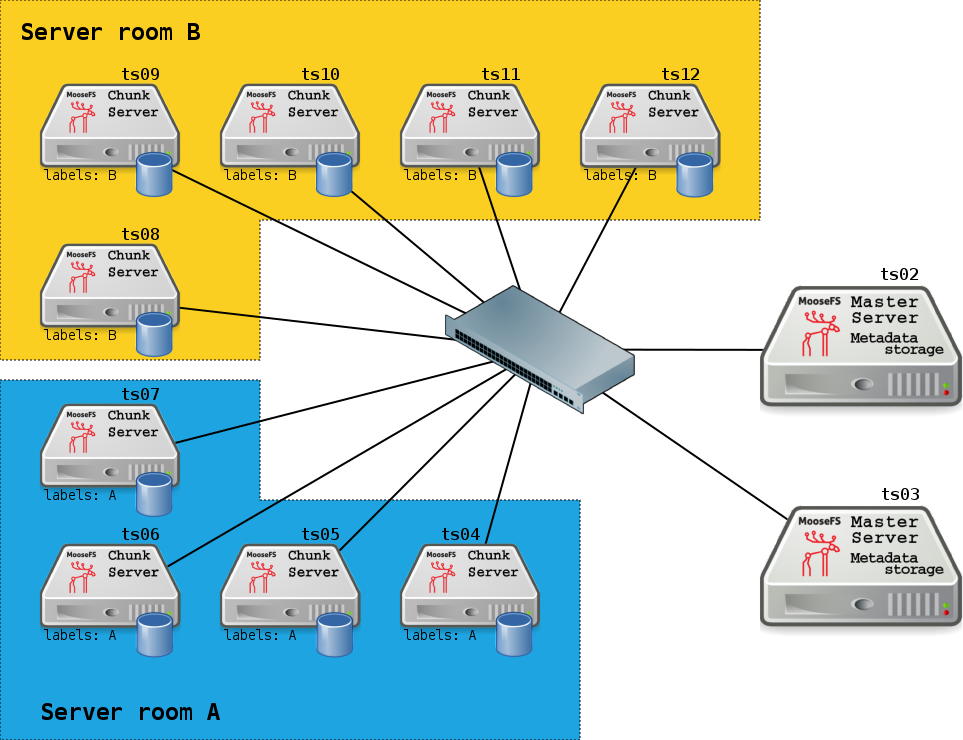
\includegraphics[scale=0.47]{images/diagram_A_B_v2.png}
			
			Using Storage Classes, you can simply decide, which server room your data is stored to.
	
			\underline{Notice}: Slow link between the sites (server room A and server room B in above example) will slow down I/O write operations to files with chunks stored in both sites due to synchronous nature of I/O write operations. Because of that reason alone, it is recommended to have a very fast connection between sites.
			
			\pagebreak			
			
			\subsection{Scenario 2: SSD and HDD drives}
	
			Let's assume, that chunkservers ts04..ts07 have SSD drives and chunkservers ts08..ts12 have HDD drives. For example, you can label chunkservers with HDD drives as \code{H}, and with SSD drives -- as \code{S}:
			
			
			\bigskip
			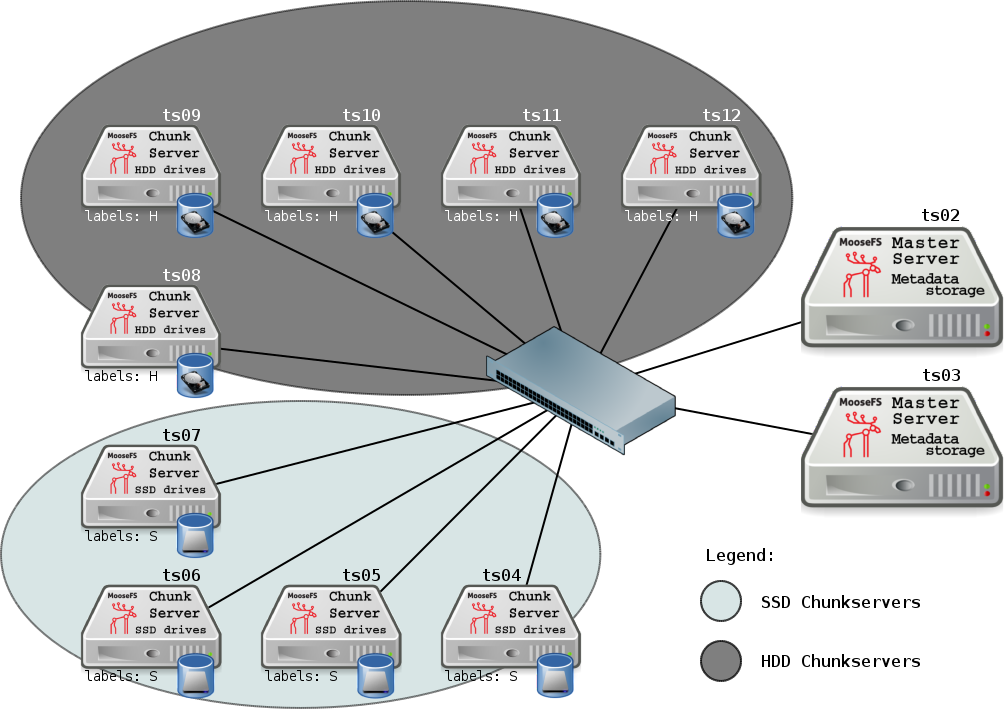
\includegraphics[scale=0.5]{images/diagram_ssd_hdd_v2.png}
			
			\bigskip
			You can configure Storage Classes, so that your frequently used data is stored on SSD Chunkservers (e.g. Storage Class \code{ssd}), and data not accessed very often  -- on HDD Chunkservers (e.g. Storage Class \code{hdd}).
			
			You can also easily move some data (e.g. after end of the year) from SSD to HDD chunkservers -- you just need to change the Storage Class assignment from \code{ssd} to \code{hdd} for this data and MooseFS will automatically take care of moving process.
			
			\underline{Example}: you have a directory named \code{Reports2015} located on MooseFS mountpoint. This directory and its subdirectories and files are used very often by a lot of processes. You want to:
			
			\begin{itemize}
				\item store this directory in four copies -- these are very important files
				\item speed up access to this directory,
			\end{itemize}
			
			so you set up and define a Storage Class e.g. \code{4ssdcopies} defined as \code{4S} (four copies on Chunkservers with fast, SSD drives) and assign it to the directory recursively. Issue the commands below:
			
			\begin{lstlisting}
			root@client:~# cd /mnt/mfs
			
			root@client:/mnt/mfs# mfsscadmin create 4S 4ssdcopies
			create ; 0
			storage class make 4ssdcopies: ok
			
			root@client:/mnt/mfs# mfssetsclass -r 4ssdcopies Reports2015
			Reports2015:
			 inodes with storage class changed:              5685
			 inodes with storage class not changed:          0
			 inodes with permission denied:                  0
			 
			root@client:/mnt/mfs#
			\end{lstlisting}
			
			But year 2015 has passed, and now \code{Reports2015} is used infrequently and you want to free some space on SSD drives to store new data. So you want to move this directory, its subdirectories and files to HDD drives and store it only in three copies.
			
			You just need to set up and define a Storage Class e.g. \code{3hddcopies} defined as \code{3H} (three copies on Chunkservers with HDD drives) and exchange the Storage Class for files which currently have \code{4ssdcopies} Storage Class applied with \code{3hddcopies} Storage Class:
			
			\begin{lstlisting}
			root@client:~# cd /mnt/mfs
			
			root@client:/mnt/mfs# mfsscadmin create 3H 3hddcopies
			create ; 0
			storage class make 3hddcopies: ok
			
			root@client:/mnt/mfs# mfsxchgsclass -r 4ssdcopies 3hddcopies Reports2015
			Reports2015:
			 inodes with storage class changed:              5685
			 inodes with storage class not changed:          0
			 inodes with permission denied:                  0
			 
			root@client:/mnt/mfs#
			\end{lstlisting}
			
			MooseFS takes care of moving process and your data is safe and accessible during moving from SSD to HDD drives (Chunkservers).
	
			\pagebreak
			
			\subsection{Scenario 3: Two server rooms (A and B) + SSD and HDD drives}
			
			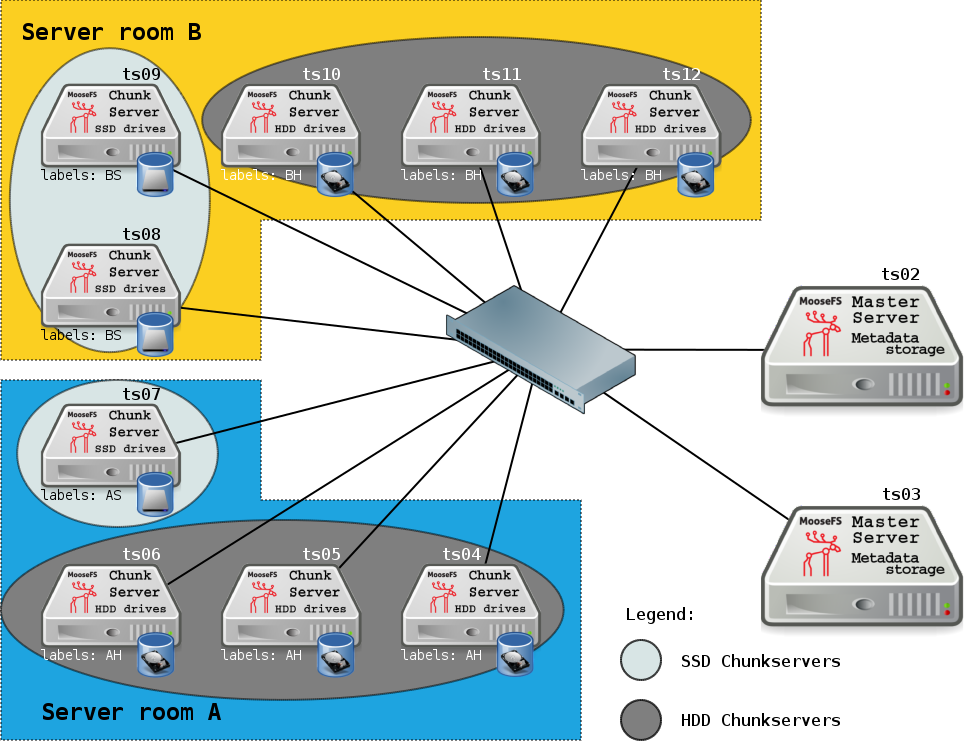
\includegraphics[scale=0.5]{images/diagram_A_B_ssd_hdd_v2.png}
	
			As shown in the picture above, this Scenario is a combination of Scenario 1 and Scenario 2. Let's assume, that in two server rooms you have two types of chunkservers: some of them containing HDD drives, some -- SSD drives.
			
			Now you want to store e.g. frequently used data on chunkservers with SSD drives and data used from time to time -- on chunkservers with HDD drives. You also want to have a copy of all data in each server room.
			
			In scenario presented above, you need to set the following labels:
			\begin{itemize}
				\item Server room A, SSD chunkservers: labels \code{A} and \code{S},
				\item Server room A, HDD chunkservers: labels \code{A} and \code{H},
				\item Server room B, SSD chunkservers: labels \code{B} and \code{S},
				\item Server room B, HDD chunkservers: labels \code{B} and \code{H}.
			\end{itemize}
			
			Then you need to set up and define appropriate Storage Classes and apply them to your files.
	
			Directory used very often named \code{Frequent} -- you want to store it in 2 copies on \textbf{SSD} drives (Chunkservers): one copy in server room \code{A}, another in server room \code{B}.
	
			\begin{lstlisting}
			root@client:~# cd /mnt/mfs
			
			root@client:/mnt/mfs# mfsscadmin create AS,BS frequent
			create ; 0
			storage class make frequent: ok
			
			root@client:/mnt/mfs# mfssetsclass -r frequent Frequent
			Frequent:
			 inodes with storage class changed:              564513
			 inodes with storage class not changed:          0
			 inodes with permission denied:                  0
			 
			root@client:/mnt/mfs#
			\end{lstlisting}
			
			Directory used from time to time named \code{Rare} -- you want to store it in 2 copies on \textbf{HDD} drives (Chunkservers): one copy in server room \code{A}, another in server room \code{B}.
			
			\begin{lstlisting}
			root@client:~# cd /mnt/mfs
			
			root@client:/mnt/mfs# mfsscadmin create AH,BH rare
			create ; 0
			storage class make rare: ok
			
			root@client:/mnt/mfs# mfssetsclass -r rare Rare
			Rare:
			 inodes with storage class changed:              497251
			 inodes with storage class not changed:          0
			 inodes with permission denied:                  0
			 
			root@client:/mnt/mfs#
			\end{lstlisting}
			
			
			So your directory \code{Frequent} (and its subdirectories and files) is stored now on Chunkservers which have both \code{A} and \code{S} labels and on Chunkservers having both \code{B} and \code{S} labels.
			
			Your directory \code{Rare} (and its subdirectories and files) is stored now on Chunkservers which have both \code{A} and \code{H} labels and on Chunkservers having both \code{B} and \code{H} labels.
			
			You also want to store your directory named \code{Backup} in three copies. You want to store one copy in server room \code{A} on SSD chunkservers, and two copies in server room \code{B}, either on HDD or SSD chunkservers. Issue the following commands:
			
			\begin{lstlisting}
			root@client:~# cd /mnt/mfs
			
			root@client:/mnt/mfs# mfsscadmin create AS,2B[H+S] backup
			create ; 0
			storage class make backup: ok
			
			root@client:/mnt/mfs# mfssetsclass -r backup Backup
			Backup:
			 inodes with storage class changed:              879784
			 inodes with storage class not changed:          0
			 inodes with permission denied:                  0
			 
			root@client:/mnt/mfs#
			\end{lstlisting}
			
			The labels expression \code{AS,2B[H+S]} is a \textit{multiplication} and \textit{sum} of labels. For more information, refer to \textbf{Section \ref{section:labels-expressions}:  \nameref{section:labels-expressions}} of this document.
			
			
			\bigskip
	
			For more information about \code{mfsscadmin} and \code{mfssetsclass}, refer to \textbf{Chapter \ref{chapter:storage-classes-tools}: \nameref{chapter:storage-classes-tools}} of this document.
	
			\underline{Notice}: Slow link between the sites (server room A and server room B in above example) will slow down I/O write operations to files with chunks stored in both sites due to synchronous nature of I/O write operations. Because of that reason alone, it is recommended to have a very fast connection between sites.
	
			
			\subsection{Scenario 4: Creation, Keep and Archive modes}
	
			Let's assume you want to write fast a big amount of important data and your computer is located closer to server room A than to server room B. So you want to create chunks in server room A, on SSD chunkservers, in two copies (\code{-C 2AS}).
	
			But your goal is to have one copy of this data in server room A, and the other one in server room B, both on SSD chunkservers. MooseFS will take care of the replication process (\code{-K AS,BS}).
			
			And finally, after 30 days, you want MooseFS to move this data to HDD chunkservers in both server room A and B (\code{-A AH,BH -d 30}).
			
			First of all, create a directory:
			
			\begin{lstlisting}
			root@client:~# cd /mnt/mfs
			root@client:/mnt/mfs# mkdir ImportantFiles
			\end{lstlisting}
			
			Then, set up and define a Storage Class, e.g. \code{important}, defined as \code{-C 2AS -K AS,BS -A AH,BH -d 30} and assign it to the newly created directory directory:
			
			\begin{lstlisting}
			root@client:~# cd /mnt/mfs
			
			root@client:/mnt/mfs# mfsscadmin create -C 2AS -K AS,BS -A AH,BH -d 30 important
			create ; 0
			storage class make important: ok
			
			root@client:/mnt/mfs# mfssetsclass important ImportantFiles
			ImportantFiles:
			 inodes with storage class changed:              1
			 inodes with storage class not changed:          0
			 inodes with permission denied:                  0
			 
			root@client:/mnt/mfs#
			\end{lstlisting}
			
			And that's all! Now you can write the data to this directory.
			
			Your data will be safe, stored very fast on SSD chunkservers in server room A while creating (you are close to this server room), copied by MooseFS also to server room B and after 30 days -- automatically moved to HDD chunkservers.
			
	\chapter{Troubleshooting}
	
		\section{Metadata save}
		Sometimes MFS master server freezes during the metadata save. To overcome this problem you should change one setting in your system. On your master machines, you should enable overcommit memory setting by issuing the following command as root:

		\begin{lstlisting}
	# echo 1 > /proc/sys/vm/overcommit_memory
		\end{lstlisting}

		To do it permanently, you can add the following line to your \code{/etc/sysctl.conf} file (it works only on Linux):

		\begin{lstlisting}
	vm.overcommit_memory=1
		\end{lstlisting}

		More detail about the reasons for this behavior:\\
		Master server performs a fork operation, effectively spawning another process to save metadata to disk. Theoretically, when you fork a process, the process memory is copied. In real life it is done the lazy way -- the memory is marked, so that if any changes are to occur, a block with changes is copied as needed, but only then. Now, if you fork a process that has 180GB of memory in use, the system can "just do it", or check if it has 180GB of free memory and reserve it for the forked "child", and only then do it and, when it doesn't have enough memory, the fork operation fails -- this is the case in Linux, so actually saving metadata is done in the main process, because fork operation failed.

		This behavior differs between systems and even between distributions of one system.

		It is safe to enable overcommit memory (the "just do it" way) with mfsmaster, because the forked process is short lived. It terminates as soon as it manages to save metadata, and during the time that it works, there are usually not that many changes to the main process' memory, so the amount of additional RAM needed is relatively small.

		Alternatively, you can add huge (at least equal to the amount of physical RAM or even more) amounts of swap space on your master servers -- then the fork should succeed, because it should always find the needed memory space in your swap.
		
		\section{Master metadata restore from Metaloggers}
		MooseFS (non-Pro) have only one Master Server, but can have several Metaloggers deployed for backup. If for some reason you loose all metadata files and changelogs from master server you can use data form metalogger to restore your data. To start dealing with recovery first you need to transfer all data stored on metalogger in \code{/var/lib/mfs} to master metadata folder. Files on metalogger will have \code{\_ml\_} prefix prepended to the filenames. After all files are copied, you need to create \code{metadata.mfs} file from changelogs and \code{metadata.back} files. To do this we need to use the command \code{mfsmaster -a}. \code{Mfsmaster} starts to build new metadata file and starts \code{mfsmaster} process.
		
		\section{Maintenance mode}
		Maintenance mode in general is helpful when there is need for maintenance on Chunkserver(s), like Chunkserver package upgrade to a newer version, adding new HDD / replacing broken ones or system upgrade (and e.g. reboot).
		
		Maintenance mode has been introduced, because in MooseFS 1.6, when there was need for maintenance on Chunkserver(s) and necessity to turn server(s) off, a lot of replications were being performed, because MooseFS had started to replicate all undergoal chunks from another available copy to fulfill the goal (it's one of MooseFS principals). Then, when it was back again -- a lot of deletions were running, because of presence of overgoal chunks, created during replications. So a lot of unnecessary I/O operations.
		
		By enabling maintenance mode before stopping Chunkserver(s) process(es) / turning machine(s) off or \textit{post factum}, you can prevent MooseFS from replicating chunks from such turned off Chunkserver(s). \textbf{Note: Server(s) in maintenance mode must match currently off (disconnected) servers. If they don't match, all chunks are replicated.}
		
		Additionally, MooseFS treats Chunkservers in maintenance mode as overloaded (no chunk creations, replications etc.). It means, that new chunks are not created on Chunkservers in maintenance mode. The reason of such behavior is because when you want to turn Chunkserver off / stop the Chunkserver process, at the moment of stopping, some I/O operations may go to this Chunkserver and when you just stop it, some write operations must be re-tried (because they haven't been finished on this stopped Chunkserver). When you turn maintenance mode on for specific Chunkserver a few seconds before stop, MooseFS will finish write operations and won't start a new ones on this Chunkserver.
		
		\textbf{Maintenance mode is designed to be a temporary state and it is not recommended to put Chunkservers in this mode for a long time.}
		
		You can enable or disable maintenance mode in CGI monitor by clicking "switch on / switch off"
		in "maintenance" column, or sending a command using:
		\begin{itemize}
			\item \code{mfscli -CM1/ip/port} -- to switch maintenance mode on
			\item \code{mfscli -CM0/ip/port} -- to switch maintenance mode off
		\end{itemize}

		\bigskip

		\textbf{Note: If number of Chunkservers in maintenance mode is equal or greater than 20\% of all Chunkserver, MooseFS treats all Chunkservers like maintenance mode wouldn't be enabled at all.}
		
		\section{Chunk replication priorities}
		In MooseFS 2.0 a few chunk replication classes and priorities have been introduced:
		\begin{itemize}
			\item Replication limit class 0 and class 1 -- replication for data safety
			\item Replication limit class 2 and class 3 -- equalization of used disk space
		\end{itemize}
		
		\bigskip
		\bigskip
		These classes and priorities are described below:		
		\bigskip		
		
		\begin{itemize}
			\item Replication limit class 0 (for endangered chunks):
				\begin{itemize}
					\item priority 0: 0 (chunk) copies on regular disks and 1 copy on disk marked for removal
					\item priority 1: 1 copy on regular disks and 0 copies on disks marked for removal
				\end{itemize}
				
			\item Replication limit class 1 (for undergoal chunks):
				\begin{itemize}
					\item priority 2: 1 copy on regular disk and some copies on disks marked for removal
					\item priority 3: $>$1 copy on regular disks and at least 1 copy on disks marked for removal
					\item priority 4: just undergoal chunks ("goal" $>$ "valid copies", no copies on disks marked for removal)
				\end{itemize}
				
			\item Replication limit class 2: Rebalancing between chunkservers with disk space usage around arithmetic mean
			\item Replication limit class 3: Rebalancing between chunkserver with disk space usage strongly above or strongly below arithmetic mean (very low or very high disk space usage, e.g. when new chunkserver is added)
		\end{itemize}
		
	\chapter{MooseFS Tools}
	
		\section{For MooseFS Master Server(s)}
		
			\subsection{\code{mfsmaster}}
				\code{mfsmaster} -- start, restart or stop Moose File System master process
				\bigskip
				
				\textbf{SYNOPSIS}
				\begin{itemize}
					\item \code{mfsmaster [-c CFGFILE] [-u] [-i] [-a] [-e] [-x[x]] [-t LOCKTIMEOUT] [ACTION]}
					\item \code{mfsmaster -v}
					\item \code{mfsmaster -h}
				\end{itemize}
				
				\bigskip
				\textbf{DESCRIPTION}
				
				\code{mfsmaster} is the master program of Moose File System.
				
				\bigskip
				
				\textbf{OPTIONS}
				\begin{itemize}
 					\item \code{-v}     print version information and exit
					\item \code{-h}     print usage information and exit
					\item \code{-c CFGFILE}
						specify  alternative path of configuration file (default is \code{mfsmaster.cfg} in system configuration directory)
					\item \code{-u}     log undefined configuration values (when default is assumed)
					\item \code{-f}     run in foreground, don't daemonize
					\item \code{-t LOCKTIMEOUT}
						how long to wait for lockfile (in seconds; default is 1800 seconds)
					\item \code{-i}     ignore some metadata structure errors
					\item \code{-a}     automatically restore metadata from change logs
					\item \code{-e}     start without metadata (usable only in pro version -- used to start additional masters)
					\item \code{-x}     produce more verbose output
					\item \code{-xx}    even more verbose output
						
					\item \code{ACTION} is  the  one  of  \code{start},  \code{stop},  \code{restart},  \code{reload}, \code{test} or \code{kill}.
						Default action is restart. The test action will yield one of two
						responses:  "\code{mfsmaster  pid: PID}" or "\code{mfsmaster is not running}".
						The kill action will send a SIGKILL  to  the  currently  running
						master  process.  SIGHUP  or  reload  action forces \code{mfsmaster} to
						reload all configuration files.
				\end{itemize}
				
				\bigskip
				\textbf{FILES}
				\begin{itemize}
					\item \code{mfsmaster.cfg}
						configuration file for MooseFS master process; refer to
						mfsmaster.cfg(5) manual for details

					\item \code{mfsexports.cfg}
						MooseFS  access  control file; refer to mfsexports.cfg(5) manual
						for details

					\item \code{mfstopology.cfg}
						Network topology definitions; refer to mfstopology.cfg(5) manual
						for details

					\item \code{.mfsmaster.lock}
						lock  file  of  running  MooseFS master process (created in data
						directory)

					\item \code{metadata.mfs}, \code{metadata.mfs.back}
						MooseFS filesystem metadata image (created in data directory)

					\item \code{changelog.*.mfs}
						MooseFS filesystem metadata change logs (created in data
						directory; merged into metadata.mfs once per hour)

					\item \code{data.stats}
						MooseFS master charts state (created in data directory)
				\end{itemize}


			\subsection{\code{mfsmetarestore}}
				\code{mfsmetarestore} -- doesn't exist this version of MooseFS
				\bigskip
				
				\textbf{DESCRIPTION}
				
				This tool was removed as of version 1.7. To achieve the same effect, simply start your mfsmaster with \code{-a} parameter.
			
			\subsection{\code{mfsmetadump}}
				\code{mfsmetadump} -- dump MooseFS metadata info in human readable format.
				\bigskip
				
				\textbf{SYNOPSIS}
				
				\code{mfsmetadump metadata\_file}
				\bigskip
				
				\textbf{DESCRIPTION}				
				\code{mfsmetadump} dumps MooseFS metadata info in human readable format.  Output consists of several sections with different types of information. Every section consist of header data -- rows starting with hash (\#) sign - and content data (may be empty).
				\newpage
				
				\textbf{FILE HEADER}
				\begin{itemize}
					\item \code{mfsmaster.cfg}
						configuration file for MooseFS master process; refer to
						mfsmaster.cfg(5) manual for details
					\item \code{header}              -- MooseFS version
					\item \code{version}             -- metadata file version
					\item \code{fileid}              -- metadata file id
				\end{itemize}
				\bigskip
				
				\textbf{SECTION HEADER}
				\begin{itemize}
					\item \code{section header}      -- section header (section type + version)
					\item \code{length}              -- length of section
					\item \code{section type}        -- name of section
					\item \code{version}             -- hexadecimal representation of section version
				\end{itemize}
				\bigskip
				
				\textbf{SESS SECTION}
				\begin{itemize}
					\item \code{nextsessionid}       -- first free session id
					\item \code{statscount}          -- number of stats remembered in each session
					\item \code{SESSION}   -- line describing a single session
					\begin{itemize}
						\item \code{s}      -- session id
						\item \code{p}      -- IP address
						\item \code{r}      -- root inode number
						\item \code{f}      -- session flags
						\item \code{g}      -- mingoal and maxgoal
						\item \code{t}      -- mintrashtime and maxtrashtime
						\item \code{m}      -- maproot uid,gid and mapall uid,gid
						\item \code{d}      -- disconnection time (optional)
						\item \code{c}      -- current hour stats data
						\item \code{l}      -- last hour stats data
						\item \code{i}      -- session name (usually local mount point)
					\end{itemize}
				\end{itemize}
				\bigskip
				
				\textbf{NODES SECTION}
				\begin{itemize}
					\item \code{maxinode}            -- maximum inode number used by system
					\item \code{hashelements}        -- number of inodes in hash table
					\item \code{NODE}      -- line with node (inode) description
					\begin{itemize}
						\item \code{k}      -- node type (-,D,S,F,B,C,L,T,R)
						\begin{itemize}
							\item \code{-}      -- file
							\item \code{D}      -- directory
							\item \code{S}      -- socket
							\item \code{F}      -- fifo
							\item \code{B}      -- block device
							\item \code{C}      -- character device
							\item \code{L}      -- symbolic link
							\item \code{T}      -- trash file
							\item \code{R}      -- sustained file (removed open file)
						\end{itemize}
						\item \code{i}      -- inode number
						\item \code{\#}      -- labelset number (10+) or goal (1-9)
						\item \code{e}      -- flags
						\item \code{m}      -- mode
						\item \code{u}      -- uid
						\item \code{g}      -- gid
						\item \code{a,m,c}  -- atime, mtime and ctime timestamps
						\item \code{t}      -- trashtime
						\item \code{d}      -- rdevhi,rdevlo (only block and character devices)
						\item \code{p}      -- path (only symbolic links)
						\item \code{l}      -- file length (only files)
						\item \code{c}      -- chunk list (only files)
						\item \code{r}      -- sessions that have this file open (only files)
					\end{itemize}
				\end{itemize}
				\bigskip
				
				\textbf{EDGES SECTION}
				\begin{itemize}
					\item \code{nextedgeid}          -- next available edge id (descending)
					\item \code{EDGE}      -- line with edge description
					\begin{itemize}
						\item \code{p}      -- parent inode number
						\item \code{c}      -- child inode number
						\item \code{i}      -- edge id
						\item \code{n}      -- edge name
					\end{itemize}
				\end{itemize}
				\bigskip
				
				\textbf{FREE SECTION}
				\begin{itemize}
					\item \code{free nodes}          -- number of free (reusable) nodes
					\item \code{FREEID}    -- line with free inode description
					\begin{itemize}
						\item \code{i}      -- inode number
						\item \code{f}      -- deletion timestamp
					\end{itemize}
				\end{itemize}
				\bigskip
				
				\textbf{QUOTA SECTION}
				\begin{itemize}
					\item \code{quota nodes}         -- number of nodes with quota
					\item \code{QUOTA}     -- line with quota description
					\begin{itemize}
						\item \code{i}      -- inode number
						\item \code{g}      -- grace period
						\item \code{e}      -- exceeded
						\item \code{f}      -- flags
						\item \code{s}      -- soft quota exceeded timestamp
						\item \code{si}     -- soft inode quota
						\item \code{hi}     -- hard inode quota
						\item \code{sl}     -- soft length quota
						\item \code{hl}     -- hard length quota
						\item \code{ss}     -- soft size quota
						\item \code{hs}     -- hard size quota
						\item \code{sr}     -- soft real size quota
						\item \code{hr}     -- hard real size quota
					\end{itemize}
				\end{itemize}
				\bigskip
				
				\textbf{XATTR SECTION}
				\begin{itemize}
					\item \code{XATTR}     -- line with xattr description
					\begin{itemize}
						\item \code{i}      -- inode number
						\item \code{n}      -- xattr name
						\item \code{v}      -- xattr value
					\end{itemize}
				\end{itemize}
				\bigskip
				
				\textbf{POSIX ACL SECTION}
				\begin{itemize}
					\item \code{POSIXACL}  -- line with acl description
					\begin{itemize}
						\item \code{i}      -- inode number
						\item \code{t}      -- acl type
						\item \code{u}      -- user (file owner) permissions
						\item \code{g}      -- group permissions
						\item \code{o}      -- other permissions
						\item \code{m}      -- permission mask
						\item \code{n}      -- named permissions -- list of objects:
						\begin{itemize}
							\item \code{u(U):P}  -- permissions \code{P} for user with uid \code{U}
							\item \code{g(G):P}  -- permissions \code{P} for group with gid \code{G}
						\end{itemize}
					\end{itemize}
				\end{itemize}
				\bigskip
				
				\textbf{OPEN SECTION}
				\begin{itemize}
					\item \code{chunk servers}       -- number of chunkservers
					\item \code{CHUNKSERVER}         -- line with chunk server description
					\begin{itemize}
						\item \code{i}      -- server ip
						\item \code{p}      -- server port
						\item \code{\#}     -- server id
						\item \code{m}      -- maintenance mode
					\end{itemize}
				\end{itemize}
				\bigskip
				
				\textbf{CHUNKSERVERS SECTION}
				\begin{itemize}
					\item \code{OPENFILE}  -- line with open file description
					\begin{itemize}
						\item \code{s}      -- session id
						\item \code{i}      -- inode number
					\end{itemize}
				\end{itemize}
				\bigskip
				
				\textbf{CHUNKS SECTION}
				\begin{itemize}
					\item \code{nextchunkid}         -- first available chunk number
					\item \code{CHUNK}     -- line with chunk description
					\begin{itemize}
						\item \code{i}      -- chunk number
						\item \code{v}      -- chunk version
						\item \code{t}      -- "locked to" timestamp
						\item \code{a}      -- archive flag
					\end{itemize}
				\end{itemize}
				
		\section{For MooseFS Supervisor}
			\subsection{\code{mfssupervisor}}
				\code{mfssupervisor} -- choose or switch leader master
				
				\bigskip
				\textbf{SYNOPSIS}
				\begin{itemize}
					\item \code{mfssupervisor [-xdfi] [-l new leader ip] [-H master host name]} \\ \code{[-P master supervising port]}
					\item \code{mfssupervisor -v}
					\item \code{mfssupervisor -h}
				\end{itemize}
				
				\bigskip
				\textbf{DESCRIPTION} \\\\
					\code{mfssupervisor} is the supervisor program of Moose  File  System.  It  is
					needed  to start a completely new system or a system after a big crash.
					It can be also used to force select a new leader master.
				
				\bigskip
				\textbf{OPTIONS}
				\begin{itemize}
					\item \code{-v} -- print version information and exit
					\item \code{-h} -- print usage information and exit
					\item \code{-x} -- produce more verbose output
					\item \code{-d} -- dry run (print info, but do not change anything)
					\item \code{-f} -- force electing not synchronized follower;  use  this  option  to initialize a new system
					\item \code{-i} -- print info only about masters state
					\item \code{-l} -- try to switch current leader to given ip
					\item \code{-H} -- use given host to find your master servers (default: \code{mfsmaster})
					\item \code{-P} -- use given port to connect to your master servers (default: \code{9419})
				\end{itemize}
		\section{For MooseFS Command Line Interface}
			\subsection{\code{mfscli}}
				\code{mfscli} -- CGI in TXT mode
				\bigskip
				
				\textbf{SYNOPSIS}
				\begin{itemize}
					\item \code{/usr/bin/mfscli [-pn28] [-H master\_host] [-P master\_port] [-f 0..3] \\
					-S(IN|IM|LI|IG|MU|IC|IL|CS|MB|HD|EX|MS|MO|QU) [-s separator] [-o order\_id [-r]] [-m mode\_id]}

					\item \code{/usr/bin/mfscli [-pn28] [-H master\_host] [-P master\_port] [-f 0..3] \\
					-C(RC/ip/port|BW/ip/port|M[01]/ip/port|RS/sessionid)}
					
					\item \code{mfscli -h}
				\end{itemize}
				\bigskip
				
				\textbf{DESCRIPTION}
				
				\code{mfscli} is a commandline counterpart to MooseFS's CGI interface. All the information available in CGI (except for graphs) can be obtained via CLI using different "monitoring options"
				\bigskip
				
				\textbf{OPTIONS}:
				\begin{itemize}
					\item \code{-h} -- print help message
					\item \code{-p} -- force plain text format on tty devices
					\item \code{-n} -- do not resolve ip adresses (default when output device is not tty)
					\item \code{-s separator} -- field separator to use in plain text format on tty devices (forces -p)
					\item \code{-2} -- force 256-color terminal color codes
					\item \code{-8} -- force 8-color terminal color codes
					\item \code{-H} master\_host -- master address (default: mfsmaster)
					\item \code{-P} master\_port -- master client port (default: 9421)

					\item \code{-f 0..3} -- set frame charset to be displayed as table frames in ttymode
					\begin{itemize}
						\item \code{0} -- use simple ascii frames \code{+}, \code{-}, \code{|} (default)
						\item \code{1} -- thick unicode frames
						\item \code{2} -- thin unicode frames
						\item \code{3} -- double unicode frames (dos style)
					\end{itemize}
					
					\item \code{-o order\_id} -- sort data by column specified by \code{order\_id} (depends on data set)
					\item \code{-r} -- reverse sort order
					\item \code{-m mode\_id} -- show data specified by \code{mode\_id} (depends on data set)
				\end{itemize}
				\bigskip
				
				\textbf{MONITORING OPTIONS}:
				\begin{itemize}
					\item \code{-SIN} -- show full master info
					\item \code{-SIM} -- show only masters states
					\item \code{-SLI} -- show only licence info
					\item \code{-SIG} -- show only general master (leader) info
					\item \code{-SIC} -- show only chunks info (goal/copies matrices)
					\item \code{-SIL} -- show only loop info (with messages)
					\item \code{-SCS} -- show connected chunk servers
					\item \code{-SMB} -- show connected metadata backup servers
					\item \code{-SHD} -- show hdd data
					\item \code{-SEX} -- show exports
					\item \code{-SMS} -- show active mounts
					\item \code{-SMO} -- show operation counters
					\item \code{-SQU} -- show quota info
					\item \code{-SMC} -- show master charts data
					\item \code{-SCC} -- show chunkserver charts data
				\end{itemize}
				\bigskip
				
				\textbf{COMMANDS}:
				\begin{itemize}
					\item \code{-CRC/ip/port} -- remove given chunkserver from list of active chunkservers
					\item \code{-CBW/ip/port} -- send given chunkserver back to work (from grace state)
					\item \code{-CM1/ip/port} -- switch selected chunkserver to maintenance mode
					\item \code{-CM0/ip/port} -- switch selected chunkserver to standard mode (from maintenance mode)
					\item \code{-CRS/sessionid} -- remove given session
				\end{itemize}
				\bigskip
				
				\textbf{EXAMPLES}:
				\begin{itemize}
					\item \code{mfscli -SIC -2} -- shows table with chunk state matrix (number of chunks for each combination of valid copies and goal set by user) using extended terminal colors (256-colors) chunkservers
					\item \code{mfscli -SCS -f 1} -- shows table with all chunkservers using unicode thick frames
					\item \code{mfscli -SMS -p -s ','} -- shows current sessions (mounts) using plain text format and coma as a separator
				\end{itemize}
				
		\section{For MooseFS CGI Server}
			\subsection{\code{mfscgiserv}}
				\code{mfscgiserv} -- start HTTP/CGI server for Moose File System monitoring
				\bigskip
				
				\textbf{SYNOPSIS}
				\begin{itemize}
					\item \code{mfscgiserv  [-H  BIND\_HOST] [-P BIND\_PORT] [-R ROOT\_PATH] [-t LOCKTIMEOUT] [-f [-v]] [ACTION]}
					\item \code{mfscgiserv -h}
				\end{itemize}
				\bigskip
				
				\textbf{DESCRIPTION}
				
				\code{mfscgiserv} is a very simple HTTP server capable of running CGI  scripts for Moose File System monitoring.

				\bigskip
				\textbf{OPTIONS}
				\begin{itemize}
					\item \code{-h} -- print usage information and exit
					\item \code{-H BIND\_HOST} -- local address to listen on (default: any)
					\item \code{-P BIND\_PORT} -- port to listen on (default: \code{9425})
					\item \code{-R ROOT\_PATH} -- local  path  to use as HTTP document root (default is \code{CGIDIR} set up at configure time)
					\item \code{-f} --run in foreground, don't daemonize
					\item \code{-v} -- log requests on stderr
					\item \code{-t LOCKTIMEOUT} -- how long to wait for lockfile (in seconds; default  is  60  seconds)
				\end{itemize}
				
				\bigskip				
				\code{ACTION }is  one  of  \code{start},  \code{stop},  \code{restart}  or  \code{test}. Default action is
					\code{restart}. The \code{test} action will yeld one of two responses:
					"\code{mfscgiserv pid: PID}" or "\code{mfscgiserv is not running}".
					
		\section{For MooseFS Metalogger(s)}
			\subsection{\code{mfsmetalogger}}
				\code{mfsmetalogger} -- start,  restart  or stop Moose File System metalogger process

				\bigskip
				\textbf{SYNOPSIS}
				\begin{itemize}
					\item \code{mfsmetalogger [-f] [-c CFGFILE] [-u] [-d] [-t LOCKTIMEOUT] [ACTION]}
					\item \code{mfsmetalogger -s [-c CFGFILE]}
					\item \code{mfsmetalogger -v}
					\item \code{mfsmetalogger -h}
				\end{itemize}
				
				\bigskip
				\textbf{DESCRIPTION} \\\\
				\code{mfsmetalogger} is the metadata replication server of Moose File  System.
					Depending  on parameters it can start, restart or stop MooseFS metalogger
					process.  Without any options it starts MooseFS metalogger, killing
					previously run process if lock file exists.

					\code{SIGHUP} (or '\code{reload}' \code{ACTION}) forces \code{mfsmetalogger} to reload all configuration files.
					
					\code{mfsmetalogger} exists since 1.6.5 version of MooseFS; before  this  version
					\code{mfschunkserver} was responsible of logging metadata changes.
					
				\begin{itemize}	
					\item \code{-v} -- print version information and exit
					\item \code{-h} -- print usage information and exit
					\item \code{-f} -- (\textbf{deprecated}, use start action instead) forcily run MooseFS
						metalogger process, without trying to kill previous  instance (this
						option allows to run MooseFS  metalogger  if  stale PID file
						exists)
					\item \code{-s} -- (\textbf{deprecated}, use stop action instead)  stop  MooseFS  metalogger process

					\item \code{-c CFGFILE} -- specify  alternative path of configuration file (default is \code{mfsmetalogger.cfg} in system configuration directory)
					\item \code{-u} -- log undefined configuration values (when default is assumed)
					\item \code{-d} -- run in foreground, don't daemonize
					\item \code{-t LOCKTIMEOUT} -- how long to wait for lockfile (default is 60 seconds)
				\end{itemize}
				\bigskip
				
				\code{ACTION} is the one of \code{start},  \code{stop},  \code{restart},  \code{reload},  \code{test}  or  \code{kill}. Default action is \code{restart} unless \code{-s} (stop) or \code{-f} (start) option is given. Note that \code{-s} and \code{-f} options are \textbf{deprecated}, likely to disappear and \code{ACTION} parameter to become obligatory in MooseFS 1.7+.
				\newpage
				
				\textbf{FILES}
				\begin{itemize}	
					\item \code{mfsmetalogger.cfg} -- configuration file for MooseFS metalogger process; refer to mfsmetalogger.cfg(5) manual for details
					\item \code{mfsmetalogger.lock} -- PID  file  of  running  MooseFS metalogger  process (created in \code{RUN\_PATH} by MooseFS $<$ 1.6.9)
					\item \code{.mfsmetalogger.lock} -- lock file of running MooseFS metalogger process (created in data directory since MooseFS 1.6.9)
					\item \code{changelog\_ml.*.mfs} -- MooseFS filesystem metadata change logs (backup of master change log files)
					\item \code{metadata.ml.mfs.back} -- Latest copy of complete \code{metadata.mfs.back} file from MooseFS master.
					\item \code{sessions.ml.mfs} -- Latest copy of \code{sessions.mfs} file from MooseFS master.
				\end{itemize}
				
				
		\section{For MooseFS Chunkserver(s)}
			\subsection{\code{mfschunkserver}}
				\code{mfschunkserver}  --  start, restart or stop Moose File System chunkserver process

				\bigskip
				\textbf{SYNOPSIS}
				\begin{itemize}
					\item \code{mfschunkserver [-c CFGFILE] [-u] [-f] [-t LOCKTIMEOUT] [ACTION]}
					\item \code{mfschunkserver -v}
					\item \code{mfschunkserver -h}
				\end{itemize}
				
				\bigskip
				\textbf{DESCRIPTION} \\\\
					\code{mfschunkserver} is the data server of Moose File System.

				\bigskip
				\textbf{OPTIONS}
				\begin{itemize}
					\item \code{-v} -- print version information and exit
					\item \code{-h} -- print usage information and exit
					\item \code{-c CFGFILE} -- specify alternative  path  of  configuration  file  (default  is
						\code{mfschunkserver.cfg} in system configuration directory)
					\item \code{-u} -- log undefined configuration values (when default is assumed)
					\item \code{-f} -- run in foreground, don't daemonize
					\item \code{-t LOCKTIMEOUT} -- how  long  to  wait for lockfile (in seconds; default is 60 seconds)
				\end{itemize}
				
				\bigskip
				\code{ACTION} is the one of \code{start},  \code{stop},  \code{restart},  \code{reload},  \code{test}  or  \code{kill}. Default  action is \code{restart}. The test action will yield one of two responses: "\code{mfschunkserver pid: PID}" or "\code{mfschunkserver  is  not running}".  The  kill action will send a \code{SIGKILL} to the currently running chunkserver process.  \code{SIGHUP}  or  reload  action  forces \code{mfschunkserver} to reload all configuration files.

				\bigskip					
				\textbf{FILES}
				\begin{itemize}
					\item \code{mfschunkserver.cfg} -- configuration  file  for  MooseFS  chunkserver process; refer to mfschunkserver.cfg(5) manual for details
					\item \code{mfshdd.cfg} -- list of directories  (mountpoints)  used  for  MooseFS  storage; refer to mfshdd.cfg(5) manual for details
					\item \code{.mfschunkserver.lock} -- lock  file  of  running  MooseFS chunkserver process (created in data directory)
					\item \code{data.csstats} -- chunkserver charts state (created in data directory)
				\end{itemize}
		
		\section{For MooseFS Client}
			\subsection{\code{mfsmount}}
				\code{mfsmount} -- mount Moose File System
				
				\bigskip
				\textbf{SYNOPSIS}
				\begin{itemize}
					\item \code{mfsmount  mountpoint  [-d] [-f] [-s] [-m] [-n] [-p] [-H HOST] [-P PORT] [-S PATH] [-o opt[,opt]...]}
					\item \code{mfsmount -h|--help}
					\item \code{mfsmount -V|--version}
				\end{itemize}
				
				\bigskip
				\textbf{DESCRIPTION}
				
				Mount Moose File System.
				\bigskip

				General options:
				\begin{itemize}
					\item \code{-h}, \code{--help} -- display help and exit
					\item \code{-V} -- display version information and exit
				\end{itemize}
				\bigskip
				
				FUSE options:
				\begin{itemize}
					\item \code{-d}, \code{-o debug} -- enable debug mode (implies \code{-f})
					\item \code{-f} -- foreground operation
					\item \code{-s} -- disable multi-threaded operation
				\end{itemize}
				\newpage
				
				MooseFS options:
				\begin{itemize}
					\item \code{-c CFGFILE, -o mfscfgfile=CFGFILE}
						-- loads file with additional mount options

					\item \code{-m}, \code{--meta}, \code{-o mfsmeta}
						-- mount MFSMETA companion filesystem instead of primary MooseFS

					\item \code{-n}
						-- omit default mount options (\code{-o allow\_other,default\_permissions})

					\item \code{-p}
						-- prompt for password (interactive version of \code{-o mfspassword=PASS})

					\item \code{-H HOST}, \code{-o mfsmaster=HOST}
						-- connect with MooseFS master on \code{HOST} (default is mfsmaster)

					\item \code{-P PORT}, \code{-o mfsport=PORT}
						-- connect with MooseFS master on \code{PORT} (default is 9421)

					\item \code{-B HOST}, \code{-o mfsbind=HOST}
						-- local address to use  for  connecting  with  master  instead  of
						default one

					\item \code{-S PATH}, \code{-o mfssubfolder=PATH}
						-- mount  specified  MooseFS  directory  (default  is \code{/}, i.e. whole
						filesystem)

					\item \code{-o mfspassword=PASSWORD}
						-- authenticate to MooseFS master with PASSWORD

					\item \code{-o mfsmd5pass=MD5}
						-- authenticate to MooseFS master using directly given MD5 (only if
						\code{mfspassword} option is not specified)
					
					\item \code{-o mfsdonotrememberpassword}
						-- do not remember password in memory -- more secure, but when session is lost then new session is created without password

					\item \code{-o mfsdebug}
						-- print some MooseFS-specific debugging information

					\item \code{-o mfsdelayedinit}
						-- connection with master is done in background -- with this option mount can be run without network (good for being run from fstab / init scripts etc.)

					\item \code{-o mfsmkdircopysgid=N}
						-- sgid bit should be copied during mkdir operation (default depends on operating system)

					\item \code{-o mfssugidclearmode=SMODE}
						-- set sugid clear mode (see SUGID CLEAR MODES; default depends on operating system)

					\item \code{-o mfscachemode=CMODE}
						-- set cache mode (see DATA CACHE MODES; default is AUTO)

					\item \code{-o mfscachefiles}
						-- (deprecated) preserve file data in cache (equivalent to '-o mfscachemode=YES')

					\item \code{-o mfsattrcacheto=SEC}
						-- set attributes cache timeout in seconds (default: 1.0)

					\item \code{-o mfsxattrcacheto=SEC}
						-- set extended attributes (xattr) cache timeout in seconds (default: 30.0)

					\item \code{-o mfsentrycacheto=SEC}
						-- set file entry cache timeout in seconds (default: 0.0,  i.e. no cache)

					\item \code{-o mfsdirentrycacheto=SEC}
						-- set directory entry cache timeout in seconds (default: 1.0)

					\item \code{-o mfsnegentrycacheto=SEC}
						-- set negative entry cache timeout in seconds (default: 1.0)

					\item \code{-o mfsgroupscacheto=SEC}
						-- set supplementary groups cache timeout in seconds (default: 300.0)

					\item \code{-o mfsrlimitnofile=N}
						-- try to change limit of simultaneously opened file descriptors on startup (default: 100000)

					\item \code{-o mfsnice=LEVEL}
						-- try to change nice level to specified value on startup (default: -19)

					\item \code{-o mfswritecachesize=N}
						-- specify  write  cache size in MiB (in range: 16..2048 - default: 250)

					\item \code{-o mfsioretries=N}
						-- specify  number  of  retiries  before  I/O  error  is   returned (default: 30)
				\end{itemize}
				
				\bigskip
				General mount options (see mount(8) manual):
				\begin{itemize}
					\item \code{-o rw | -o ro}
						-- Mount  file-system  in  read-write  (default)  or read-only mode respectively.

					\item \code{-o suid | -o nosuid}
						-- Enable or disable suid/sgid attributes to work.

					\item \code{-o dev | -o nodev}
						-- Enable or disable character or block special device files interpretation.

					\item \code{-o exec | -o noexec}
						-- Allow or disallow execution of binaries.
				\end{itemize}
				\bigskip
				
				\textbf{SUGID CLEAR MODE}
				
				During attribute change file systems sometimes clear flags suid and/or sgid.  Behavior is different on different file systems.  MFS tries to mimic behavior of most popular file system on given operating systems.

					\begin{itemize}
						\item \code{NEVER}  -- MFS will not change suid and sgid bit on chown
						\item \code{ALWAYS} -- clear suid and sgid on every chown - safest operation
						\item \code{OSX}    -- standard behavior in OS X and Solaris (chown made by unprivileged user clear suid and sgid)
						\item \code{BSD}    -- standard behavior in *BSD systems (like in OSX, but only when something is really changed)
						\item \code{EXT}    -- standard behavior in most file systems on Linux (directories not changed, others: suid cleared always, sgid only when group exec bit is set)
						\item \code{XFS}    -- standard behavior in XFS on Linux (like EXT but directories are changed by unprivileged users)			
				\end{itemize}
				\bigskip
				
				\textbf{DATA CACHE MODES}
				
				There  are  three cache modes: \code{NO}, \code{YES} and \code{AUTO}. Default option is \code{AUTO} and you shouldn't change it unless you really know what you are doing. In AUTO mode data cache is managed automatically by \code{mfsmaster}.

					\begin{itemize}
						\item \code{NO}, \code{NONE} or \code{NEVER} -- never allow files data to be kept in cache (safest but can reduce efficiency)
						\item \code{YES} or \code{ALWAYS} -- always allow files data to be kept in cache (dangerous)
						\item \code{AUTO} -- file cache is managed by \code{mfsmaster} automatically (should be very safe and efficient)
				\end{itemize}
					
					
			\subsection{\code{mfstools}}
				\code{mfstools} -- perform MooseFS-specific operations
				\bigskip
				
				\textbf{SYNOPSIS}
				\begin{itemize}
					\item \code{mfsgetgoal [-r] [-n|-h|-H|-k|-m|-g] OBJECT...}
					\item \code{mfsrgetgoal [-n|-h|-H|-k|-m|-g] OBJECT...}
					\item \code{mfssetgoal [-r] [-n|-h|-H|-k|-m|-g] [+|-]N OBJECT...}
					\item \code{mfsrsetgoal [-n|-h|-H|-k|-m|-g] [+|-]N OBJECT...}
					\item \code{mfsgettrashtime [-r] [-n|-h|-H|-k|-m|-g] OBJECT...}
					\item \code{mfsrgettrashtime [-n|-h|-H|-k|-m|-g] OBJECT...}
					\item \code{mfssettrashtime [-r] [-n|-h|-H|-k|-m|-g] [+|-]SECONDS OBJECT...}
					\item \code{mfsrsettrashtime [-n|-h|-H|-k|-m|-g] [+|-]SECONDS OBJECT...}
					\item \code{mfsgeteattr [-r] [-n|-h|-H|-k|-m|-g] OBJECT...}
					\item \code{mfsseteattr  [-r]  [-n|-h|-H|-k|-m|-g]  -f  ATTRNAME  [-f ATTRNAME ...] OBJECT...}
					\item \code{mfsdeleattr [-r] [-n|-h|-H|-k|-m|-g]  -f  ATTRNAME  [-f  ATTRNAME  ...] OBJECT...}
					\item \code{mfscheckfile FILE...}
					\item \code{mfsfileinfo FILE...}
					\item \code{mfsdirinfo [-n|-h|-H|-k|-m|-g] OBJECT...}
					\item \code{mfsfilerepair [-n|-h|-H|-k|-m|-g] FILE...}
					\item \code{mfsappendchunks SNAPSHOT\_FILE OBJECT...}
					\item \code{mfsmakesnapshot [-o] SOURCE... DESTINATION}
					\item \code{mfsgetquota [-n|-h|-H|-k|-m|-g] DIRECTORY...}
					\item \code{mfssetquota  [-n|-h|-H|-k|-m|-g]  [-i|-I  inodes] [-l|-L length]
								[-s|-S size] [-r|-R realsize] DIRECTORY...}
					\item \code{mfsdelquota  [-a|-A|-i|-I|-l|-L|-s|-S|-r|-R]   [-n|-h|-H|-k|-m|-g]
								-f DIRECTORY...}
					\item \code{mfsfilepaths OBJECT|INODE...}
				\end{itemize}
				\bigskip
				
				\textbf{DESCRIPTION}
				
				\begin{itemize}
					\item \code{mfsgetgoal} and \code{mfssetgoal} operate on object's goal value, i.e. the number
					of copies in which all file data are stored.  It  means  that  file
					should  survive  failure  of one less chunkservers than its goal value.
					Goal must be set between \code{1} and \code{9} (note that \code{1} is strongly  unadvised).
					\code{mfsgetgoal}  prints  current  goal  value of given object(s).  \code{-r} option
					enables recursive mode, which works as usual for every given file,  but
					for every given directory additionally prints current goal value of all
					contained objects (files and directories).  \code{mfssetgoal} changes  current
					goal  value  of  given object(s). If new value is specified in \code{+N} form,
					goal value is increased to \code{N} for objects  with  lower  goal  value  and
					unchanged  for  the  rest.  Similarly, if new value is specified as \code{-N},
					goal value is decreased to \code{N} for objects with  higher  goal  value  and
					unchanged  for the rest. \code{-r} option enables recursive mode.  These tools
					can be used on any file, directory or deleted (trash) file.

					\item \code{mfsrgetgoal} and \code{mfsrsetgoal} are deprecated aliases  for  \code{mfsgetgoal  -r}
					and \code{mfssetgoal -r} respectively.

					\item \code{mfsgettrashtime}  and  \code{mfssettrashtime}  operate  on  object's  trashtime
					value, i.e. the number of seconds the  file  is  preserved  in  special
					trash directory before it's finally removed from filesystem.  Trashtime
					must be non-negative integer  value. \code{mfsgettrashtime}  prints  current
					trashtime  value of given object(s).  \code{-r} option enables recursive mode,
					which works as usual for every given file, but for every  given  directory
					additionally  prints  current  trashtime  value  of all contained
					objects  (files  and  directories).   \code{mfssettrashtime}  changes  current
					trashtime  value  of  given object(s).  If new value is specified in \code{+N}
					form, trashtime value is increased to \code{N} for objects with  lower  trashtime
					value and unchanged for the rest. Similarly, if new value is specified
					as \code{-N}, trashtime value is decreased to \code{N} for objects with  higher
					trashtime value and unchanged for the rest. \code{-r} option enables recursive
					mode.  These tools can be  used  on  any  file,  directory  or  deleted
					(trash) file.

					\item \code{mfsrgettrashtime} and  \code{mfsrsettrashtime} are deprecated aliases for \code{mfsgettrashtime -r} and \code{mfssettrashtime -r} respectively.

					\item \code{mfsgeteattr}, \code{mfsseteattr} and \code{mfsdeleattr} tools are used to get, set  or
					delete some extra attributes. Attributes are described below.

					\item \code{mfscheckfile}  checks  and  prints  number of chunks and number of chunk
					copies belonging to specified file(s).  It can be  used  on  any  file,
					included deleted (trash).

					\item \code{mfsfileinfo}  prints  location (chunkserver host and port) of each chunk
					copy belonging to specified file(s).  It  can  be  used  on  any  file,
					included deleted (trash).

					\item \code{mfsdirinfo}  is  extended, MooseFS-specific equivalent of \code{du -s} command.
					It prints summary for each specified object (single file  or  directory
					tree). If you only want to see one parameter, then add one of show options (see SHOW OPTIONS)

					\item \code{mfsfilerepair}  deals with broken files (those which cause I/O errors on
					read operations) to make them partially readable. In  case  of  missing
					chunk  it fills missing parts of file with zeroes; in case of chunk version
					mismatch it sets chunk version known to \code{mfsmaster} to  highest  one
					found  on  chunkservers.  Note: because in the second case content mismatch
					can occur in chunks with the same version, it's advised to make a
					copy (not a snapshot!)  and delete original file after "repairing".

					\item \code{mfsappendchunks}  (equivalent of \code{mfssnapshot} from MooseFS 1.5) appends a
					lazy copy of specified file(s) to specified snapshot file ("lazy" means
					that  creation of new chunks is delayed to the moment one copy is modified).
					If multiple files are given, they are merged  into  one  target
					file in the way that each file begins at chunk (64MB) boundary; padding
					space is left empty.

					\item \code{mfsmakesnapshot} makes a "real" snapshot (lazy copy, like  in  case  of
					\code{mfsappendchunks})  of some object(s) or subtree (similarly to \code{cp -r command}).
					It's atomic with respect to each \code{SOURCE} argument separately.  If
					\code{DESTINATION}  points  to  already  existing file, error will be reported
					unless \code{-o} (overwrite) option is given. Note: if \code{SOURCE} is a  directory,
					it's  copied  as  a whole; but if it's followed by trailing slash, only
					directory content is copied.

					\item \code{mfsgetquota}, \code{mfssetquota} and  \code{mfsdelquota}  tools  are  used  to  check,
					define and delete quotas. Quota is set on a directory. It can be set in
					one of 4 ways: for number of inodes inside the directory (total sum  of
					the  subtree's  inodes)  with \code{-i}, \code{-I} options, for sum of (logical) file
					lengths with \code{-l}, \code{-L} options, for sum of chunk  sizes  (not  considering
					goals)  with  \code{-s},  \code{-S}  options and for physical hdd space (more or less
					chunk sizes multiplied by goal of each  chunk)  with  \code{-r},  \code{-R}  options.
					Small letters set soft quota, capital letters set hard quota. \code{-a} and \code{-A}
					options in \code{mfsdelquota} mean all kinds  of  quota.  Quota  behavior  is
					described below.
					
					\item \code{mfsfilepaths} tool can be used to find all occurrences (hard links) of given file in filesystem.  Also can be used to find file by number of i-node. In case of searching by i-node tool has to be run in mfs mounted directory.
				\end{itemize}
				\bigskip
				
				\textbf{GENERAL OPTIONS}
				
					Most of mfstools use \code{-n}, \code{-h}, \code{-H}, \code{-k}, \code{-m} and \code{-g} options to select format
					of printed numbers. \code{-n} causes to print exact numbers,  \code{-h}  uses  binary
					prefixes  (\code{Ki}, \code{Mi}, \code{Gi} as $2^{10}$, $2^{20}$ etc.) while \code{-H} uses \code{SI} prefixes (\code{k},
					\code{M}, \code{G} as $10^3$, $10^6$ etc.). \code{-k}, \code{-m} and \code{-g} show plain numbers respectivaly
					in  kibis  (binary kilo -- 1024), mebis (binary mega -- $1024^2$) and gibis
					(binary giga -- $1024^3$).  The same can be achieved by setting  \code{MFSHRFORMAT}
					environment  variable  to:  0 (exact numbers), \code{1} or \code{h} (binary prefixes),
					\code{2} or \code{H} (\code{SI} prefixes), \code{3} or \code{h+} (exact numbers  and  binary  prefixes),
					\code{4}  or  \code{H+}  (exact  numbers and SI prefixes). The default is to
					print just exact numbers.
				\bigskip
				
				\textbf{SHOW OPTIONS}
				\begin{itemize}
					\item \code{-i}     -- show number of inodes
					\item \code{-d}     -- show number of directories
					\item \code{-f}     -- show number of files
					\item \code{-c}     -- show number of chunks
					\item \code{-l}     -- show length
					\item \code{-s}     -- show size
					\item \code{-r}     -- show realsize
				\end{itemize}
				\bigskip
				
				\textbf{EXTRA ATTRIBUTES}
				\begin{itemize}
					\item \code{noowner} -- This flag means, that particular object belongs to current user
					(\code{uid}  and  \code{gid}  are  equal to \code{uid} and \code{gid} values of accessing process). Only \code{root} (\code{uid=0}) sees the real \code{uid} and \code{gid}.

					\item \code{noattrcache} -- This flag means, that standard file attributes such as \code{uid}, code{gid}, \code{mode}, \code{length} and so on won't be stored in kernel cache. In MooseFS 1.5  this  was  the  only  behavior,  and  \code{mfsmount}  always  prevented attributes  from  being  stored  in  kernel  cache,  but in MooseFS 1.6 attributes can be cached, so in very rare ocassions it could be  useful to turn it off.

					\item \code{noentrycache} --  This  flag  is  similar  to  above. It prevents directory entries from being cached in kernel.
				\end{itemize}
				\bigskip
				
				\textbf{QUOTAS}
				
					Quota is always set on a directory. Hard quota cannot be exceeded  any
					time.  Soft quota can be exceeded for a period of time (7 days). Once a
					quota is exceeded in a directory, user must go below the  quota  during
					the  next  7 days. If not, the soft quota for this particular directory
					starts to behave like a hard quota. The 7 days  period  is  global  and
					cannot currently be modified.
				\bigskip
				
				\textbf{INHERITANCE}
				
					When  new object is created in MooseFS, attributes such as \code{goal}, \code{trashtime}
					and extra attributes are inherited from parent  directory.  So  if
					you  set  i.e.  "\code{noowner}"  attribute  and \code{goal} to \code{3} in a directory then
					every new object created in this directory will have \code{goal} set to \code{3}  and
					"\code{noowner}"  flag set. A newly created object inherits always the current
					set of its parent's attributes. Changing a directory attribute does not
					affect  its  already  created  children.  To  change an attribute for a
					directory and all of its children use "\code{-r}" option.
	
	\chapter{MooseFS Configuration Files}
		\section{For MooseFS Master Server(s)}
			\bigskip
			\begin{center}
				\textbf{\fcolorbox{red}{pink}{Warning: Configuration files on all Master Servers must be consistent!}}
			\end{center}
			\bigskip
			
			\subsection{\code{mfsmaster.cfg}}
				\code{mfsmaster.cfg} -- main configuration file for \code{mfsmaster}

				\bigskip
				\textbf{DESCRIPTION} \\\\
					The   file  \code{mfsmaster.cfg}  contains  configuration  of  MooseFS  master
					process.

				\bigskip
				\textbf{SYNTAX} \\\\
				Syntax is:
				
				\code{OPTION = VALUE}

				Lines starting with \code{\#} character are ignored as comments.
				
				\bigskip
				\textbf{OPTIONS} \\\\
				Configuration options:
				\begin{itemize}
					\item \code{WORKING\_USER}
						-- user to run daemon as

					\item \code{WORKING\_GROUP}
						-- group to run daemon as; optional value - if empty  then  default
						user group will be used

					\item \code{SYSLOG\_IDENT}
						-- name  of process to place in syslog messages; default is \code{mfsmaster}

					\item \code{LOCK\_MEMORY}
						-- whether to perform mlockall() to avoid  swapping  out  \code{mfsmaster}
						process; default is 0, i.e. no

					\item \code{NICE\_LEVEL}
						-- nice  level  to  run  daemon with; default is -19; note: process
						must be started as root to increase priority, if setting of
						priority fails, process retains the nice level it started with

					\item \code{FILE\_UMASK}
						-- set  default  umask  for  group  and others (user has always 0);
						default is \code{027} -- block write for group and block all for others

					\item \code{DATA\_PATH}
						-- where to store metadata files and lock file

					\item \code{EXPORTS\_FILENAME}
						-- alternate location/name of \code{mfsmaster.cfg} file

					\item \code{TOPOLOGY\_FILENAME}
						-- alternate location/name of \code{mfstopology.cfg} file
						
					\item \code{LICENCE\_FILENAME}
						-- alternate location/name of \code{mfslicence.bin} file (pro version only)

					\item \code{BACK\_LOGS}
						-- number of metadata change log files (default is 50)

					\item \code{BACK\_META\_KEEP\_PREVIOUS}
						-- number of previous metadata files to be kept (default is 1)

					\item \code{CHANGELOG\_PRESERVE\_SECONDS}
						-- how many seconds of change logs have to be preserved  in  memory
						(default  is 1800; this sets the minimum, actual number may be a
						bit bigger due to logs being kept in 5k  blocks;  zero  disables
						extra logs storage)
						
					\item \code{MISSING\_LOG\_CAPACITY}
						-- how many missing chunks will be stored in master (up to \\ \code{100*MISSING\_LOG\_CAPACITY} bytes of memory will be allocated; default value is 100000)

					\item \code{MATOML\_LISTEN\_HOST}
						-- IP  address to listen on for \code{metalogger}, \code{master}s and \code{supervisor}s connections (* means any)

					\item \code{MATOML\_LISTEN\_PORT}
						-- port to listen on for \code{metalogger}, \code{master}s and  \code{supervisor}s  connections

					\item \code{MASTER\_RECONNECTION\_DELAY}
						-- delay in  seconds before next try to reconnect to \code{master-leader}
						if not connected (default is 5)

					\item \code{MASTER\_TIMEOUT}
						-- timeout in seconds for \code{master-leader} connections (pro version only; default is 10)

					\item \code{BIND\_HOST}
						-- local address to use for connecting with \code{master-leader} (pro version only; default is *, i.e. default local address)

					\item \code{MATOCS\_LISTEN\_HOST}
						-- IP  address  to  listen  on for \code{chunkserver} connections (\code{*} means any)

					\item \code{MATOCS\_LISTEN\_PORT}
						-- port to listen on for \code{chunkserver} connections
						
					\item \code{MATOCS\_TIMEOUT}
						-- timeout in seconds for master-chunkserver connection (default is 10)

					\item \code{REPLICATIONS\_DELAY\_INIT}
						-- initial delay in seconds before starting  replications  (default is 300)

					\item \code{CHUNKS\_LOOP\_MAX\_CPS}
						-- Chunks loop shouldn't check more chunks per seconds  than  given
						number (default is 100000)

					\item \code{CHUNKS\_LOOP\_MIN\_TIME}
						-- Chunks  loop shouldn't be done in less seconds than given number
						(default is 300)

					\item \code{CHUNKS\_SOFT\_DEL\_LIMIT}
						-- Soft maximum number of  chunks  to  delete  on  one  \code{chunkserver}
						(default is 10)

					\item \code{CHUNKS\_HARD\_DEL\_LIMIT}
						-- Hard  maximum  number  of  chunks  to  delete on one \code{chunkserver}
						(default is 25)

					\item \code{CHUNKS\_WRITE\_REP\_LIMIT}
						-- Maximum number of chunks to replicate to one \code{chunkserver} (default is 2,1,1,4 -- see NOTES)

					\item \code{CHUNKS\_READ\_REP\_LIMIT}
						-- Maximum number of chunks to replicate from one \code{chunkserver} (default is 10,5,2,5 -- see NOTES)

					\item \code{CS\_HEAVY\_LOAD\_THRESHOLD}
						-- Threshold for chunkserver load (default is 100 -- see NOTES)

					\item \code{CS\_HEAVY\_LOAD\_RATIO\_THRESHOLD}
						-- Threshold ratio for chunkserver load (default is 5.0 -- see NOTES)

					\item \code{CS\_HEAVY\_LOAD\_GRACE\_PERIOD}
						-- Defines how long chunkservers will remain in 'grace' mode (default is 900 -- see NOTES)

					\item \code{ACCEPTABLE\_DIFFERENCE}
						-- Maximum difference between space usage of chunkservers (deprecated, use \code{ACCEPTABLE\_PERCENTAGE\_DIFFERENCE} instead)
						
					\item \code{ACCEPTABLE\_PERCENTAGE\_DIFFERENCE}
						-- Maximum percentage difference between space usage of chunkservers (default is 1 = 1\%)
					\item \code{PRIORITY\_QUEUES\_LENGTH}
						-- Length of priority queues (for endangered, undergoal etc. chunks -- chunks that should be processed first -- default is 1000000)

					\item \code{MATOCL\_LISTEN\_HOST}
						-- IP address to listen on for client (mount) connections (\code{*}  means any)

					\item \code{MATOCL\_LISTEN\_PORT}
						-- port to listen on for client (mount) connections

					\item \code{SESSION\_SUSTAIN\_TIME}
						-- How  long  to sustain a disconnected client session (in seconds; default is 86400 = 1 day)

					\item \code{QUOTA\_TIME\_LIMIT}
						-- Time limit in seconds for soft quota  (default  is  604800  =  7 days)
						
					\item \code{ATIME\_MODE}
						-- Set atime modification mode (default is 0 = always modify atime -- see NOTES)
				\end{itemize}
				\bigskip
				
				\textbf{NOTES}
				
					Chunks  in  master  are tested in a loop. Speed (or frequency) is
					regulated by  two  options  \code{CHUNKS\_LOOP\_MIN\_TIME}  and  \code{CHUNKS\_LOOP\_MAX\_CPS}.
					First  defines  minimal  time between iterations of the loop and second
					defines maximal number of chunk tests per  second.   Typically  at  the
					beginning,  when number of chunks is small, time is constant, regulated
					by \code{CHUNK\_LOOP\_MIN\_TIME}, but when number of chunks becomes bigger  then
					time of loop can increase according to\\
					\code{CHUNKS\_LOOP\_MAX\_CPS}.

					Example: \code{CHUNKS\_LOOP\_MIN\_TIME} is set to 300, \code{CHUNKS\_LOOP\_MAX\_CPS} is set
					to 100000 and there is 1000000 (one  million)  chunks  in  the  system.
					1000000/100000 = 10, which is less than 300, so one loop iteration will
					take 300 seconds.  With 1000000000  (one  billion)  chunks  the  system
					needs 10000 seconds for one iteration of the loop.

					Deletion  limits are defined as 'soft' and 'hard' limit. When number of
					chunks to delete increases from loop to loop, current limit can be temporary
					increased above soft limit, but never above hard limit.
					
					Replication limits are divided into four cases:
					\begin{itemize}
						\item first limit is for endangered chunks (chunks with only one copy)
						\item second limit is for undergoal chunks (chunks with number of copies lower than specified goal)
						\item third limit is for rebalance between servers with space usage around arithmetic mean
						\item fourth limit is for rebalance between other servers (very low or very high space usage)
					\end{itemize}
					
					Usually first number should be grater than or equal to second, second greater than or equal to third, and fourth greater than or equal to third (1st $>=$ 2nd $>=$ 3rd $<=$ 4th). If one number is given, then all limits are set to this  number (for backward compatibility).

					Whenever  chunkserver  load  is  higher  than  \code{CS\_HEAVY\_LOAD\_THRESHOLD}   and \\ \code{CS\_HEAVY\_LOAD\_RATIO\_THRESHOLD}  times  higher  than  average  load,  then  chunkserver  is  switched  into  'grace'  mode. Chunkserver stays in grace mode for \code{CS\_HEAVY\_LOAD\_GRACE\_PERIOD} seconds.

       				There are five values for \code{ATIME\_MODE} (all other values are treated as \code{0}):
					\begin{itemize}
						\item \code{0} = Always modify atime for files, folders and symlinks.
						\item \code{1} = Always modify atime but only in case of files (do not modify atime in case of folders and symlinks).
						\item \code{2} = Modify atime only when it is lower than ctime or mtime and when current time is higher than ctime or mtime respectively, also modify atime when current atime is older than 24h. Do it for all objects during access (like "relatime"
         option in Linux).
						\item \code{3} = Same as above but only in case of files. In case of folders and symlinks do not modify atime.
						\item \code{4} = Never modify atime during access (like "noatime" option).
					\end{itemize}
					
			\subsection{\code{mfsexports.cfg}}
				\code{mfsexports.cfg} -- MooseFS access control for \code{mfsmount}s				
				\bigskip
				
				\textbf{DESCRIPTION}
				
				The  file  \code{mfsexports.cfg}  contains  MooseFS  access  list for \code{mfsmount} clients.
				\bigskip
				
				\textbf{SYNTAX}
				
				Syntax is:
				\code{ADDRESS DIRECTORY [OPTIONS]}

				Lines starting with \code{\#} character are ignored as comments.

				\code{ADDRESS} can be specified in several forms:
					\begin{itemize}
						\item \code{*}				-- all addresses
						\item \code{n.n.n.n}			-- single IP address
						\item \code{n.n.n.n/b}		-- IP class specified by network address and number of significant bits
						\item \code{n.n.n.n/m.m.m.m}	-- IP class specified by network address and mask
						\item \code{f.f.f.f-t.t.t.t}	-- IP range specified by from-to addresses (inclusive)
					\end{itemize}
				
				\bigskip
				\code{DIRECTORY} can be \code{/} or path relative to MooseFS root;  special  value  \code{.} means MFSMETA companion filesystem.
				
				\bigskip
				OPTIONS list:
				\begin{itemize}
					\item \code{ro}, \code{readonly} -- export tree in read-only mode; this is default
					\item \code{rw}, \code{readwrite} -- export tree in read-write mode
					\item \code{alldirs} -- allows  to  mount any subdirectory of specified directory (similarly to NFS)
					\item \code{dynamicip} -- allows reconnecting of already authenticated client from any  IP address (the default is to check IP address on reconnect)
					\item \code{ignoregid} -- disable  testing  of group access at \code{mfsmaster} level (it's still
						done at \code{mfsmount} level) -- in this case "group" and "other"
						permissions are logically added; needed for supplementary groups to
						work (\code{mfsmaster} receives only user primary group information)
					\item \code{admin} -- administrative privileges -- currently: allow changing of quota values
					\item \code{maproot=USER[:GROUP]} -- maps root (\code{uid=0}) accesses to given user and group (similarly to \code{maproot}  option  in  NFS  mounts);  \code{USER}  and \code{GROUP} can be given either as name or number; if no group is specified, \code{USER}'s  primary group  is  used. Names are resolved on \code{mfsmaster} side (see note below).
					\item \code{mapall=USER[:GROUP]} -- like above but maps all non privileged users  (\code{uid!=0})  accesses to given user and group (see notes below).
					\item \code{password=PASS}, \code{md5pass=MD5} -- requires  password  authentication  in order to access specified resource
					\item \code{minversion=VER} -- rejects access from clients older than specified
					\item \code{mingoal=N}, \code{maxgoal=N} -- specify range in which goal can be set by users
					\item \code{mintrashtime=TDUR}, \code{maxtrashtime=TDUR} -- specify range in which trashtime can be set by users
				\end{itemize}
				\bigskip
				
				Default  options  are:
				
				\code{ro},  \code{maproot=999:999},   \code{mingoal=1},   \code{maxgoal=9}, \code{mintrashtime=0}, \code{maxtrashtime=4294967295}.
				\bigskip
				
				\textbf{NOTES}
				
				\code{USER}  and \code{GROUP} names (if not specified by explicit \code{uid}/\code{gid} number) are
				resolved on \code{mfsmaster} host.

				\code{TDUR} can be specified as number without time unit (number  of  seconds)
				or  combination  of numbers with time units. Time units are: \code{W}, \code{D}, \code{H}, \code{M}, \code{S}. Order is important -- less  significant  time  units  can't  be  defined before more significant time units.  Time units are case insensitive.

				Option  \code{mapall} works  in MooseFS in different way than in NFS, because MooseFS is  using  FUSE's  "\code{default\_permissions}"  option.  When  \code{mapall} option  is  used, users see all objects with \code{uid} equal to mapped \code{uid} as their own and all other as root's objects. Similarly objects  with  \code{gid} equal  to  mapped  \code{gid}  are seen as objects with current user's primary group and all other objects as objects with group  0  (usually  wheel). With \code{mapall} option set attribute cache in kernel is always turned off.
				\bigskip

				\textbf{EXAMPLES}
				
				\begin{lstlisting}
	*					 /			ro
	192.168.1.0/24		 /			rw
	192.168.1.0/24		 /			rw,alldirs,maproot=0,password=passcode
	10.0.0.0-10.0.0.5	 /test		rw,maproot=nobody,password=test
	10.1.0.0/255.255.0.0 /public	rw,mapall=1000:1000
	10.2.0.0/16			 /			rw,alldirs,maproot=0,mintrashtime=2h30m,maxtrashtime=2w
				\end{lstlisting}
			
			\subsection{\code{mfstopology.cfg}}
				\code{mfstopology.cfg} -- MooseFS network topology definitions
				\bigskip
				
				\textbf{DESCRIPTION}
				
				The file \code{mfstopology.cfg} contains assignments of IP addresses into
					network locations (usually switch numbers). This file is optional. If your
					network  has  one  switch or decreasing traffic between switches is not
					necessary then leave this file empty.
				\bigskip
				
				\textbf{SYNTAX}
				
					Syntax is:
					
					\code{ADDRESS SWITCH-NUMBER}

					Lines starting with \code{\#} character are ignored as comments.

					\code{ADDRESS} can be specified in several forms:

					\begin{itemize}
						\item \code{*}			-- all addresses
						\item \code{n.n.n.n}		-- single IP address
						\item \code{n.n.n.n/b}		-- IP class specified by network address and bits number
						\item \code{n.n.n.n/m.m.m.m}	-- IP class specified by network address and mask
						\item \code{f.f.f.f-t.t.t.t}	-- IP range specified by from-to addresses (inclusive)
					\end{itemize}

					\code{SWITCH-NUMBER} can be specified as any positive 32-bit numer.


				\textbf{NOTES} \\\\
					If one IP belongs to more than one definition then last  definition  is
					used.

					As  for  now distance between switches is constant. So distance between
					machines is calculated as: 0 when IP numbers are the same,  1  when  IP
					numbers  are  different,  but  switch  numbers  are the same and 2 when
					switch numbers are different

					Distances are used only to sort  chunkservers  during  read  and  write
					operations.  New chunks are still created randomly. Also rebalance
					routines do not take distances into account.
			
			
		\section{For MooseFS Metalogger(s)}
			\subsection{\code{mfsmetalogger.cfg}}
				code{mfsmetalogger.cfg} -- configuration file for mfsmetalogger
				\bigskip
				
				\textbf{DESCRIPTION}
				
					The file \code{mfsmetalogger.cfg} contains configuration of MooseFS \code{metalogger} process.
				\bigskip
				
				\textbf{SYNTAX}
				
					Syntax is:

					\code{OPTION = VALUE}

					Lines starting with \code{\#} character are ignored as comments.
				\bigskip
				
				\textbf{OPTIONS}
				
				Configuration options:

				\begin{itemize}
					\item \code{DATA\_PATH} -- where to store metadata files

					\item \code{LOCK\_FILE} -- (deprecated) daemon lock/pid file

					\item \code{WORKING\_USER} -- user to run daemon as

					\item \code{WORKING\_GROUP} -- group to run daemon as (optional -- if empty  then  default  user group will be used)

					\item \code{SYSLOG\_IDENT} -- name of process to place in syslog messages (default is mfsmetalogger)

					\item \code{LOCK\_MEMORY} -- whether to perform mlockall() to avoid swapping out  mfsmetalogger process (default is 0, i.e. no)

					\item \code{NICE\_LEVEL} -- nice level to run daemon with (default is -19 if possible; note: process must be started as root to increase priority)

					\item \code{BACK\_LOGS} -- number of metadata change log files (default is 50)

					\item \code{BACK\_META\_KEEP\_PREVIOUS} -- number of previous metadata files to be kept (default is 3)

					\item \code{META\_DOWNLOAD\_FREQ} -- metadata download frequency in hours (default  is  24,  at  most \code{BACK\_LOGS}/2)

					\item \code{MASTER\_HOST} -- address  of MooseFS master host to connect with (default is mfsmaster)

					\item \code{MASTER\_PORT} -- number of MooseFS master port to connect with (default is 9420)

					\item \code{MASTER\_RECONNECTION\_DELAY} -- delay in seconds before trying to reconnect to master after disconnection (default is 30)

					\item \code{MASTER\_TIMEOUT} -- timeout (in seconds) for master connections (default is 60)
				\end{itemize}
			
		\section{For MooseFS Chunkservers}
			\subsection{\code{mfschunkserver.cfg}}
				\code{mfschunkserver.cfg} -- main configuration file for mfschunkserver
				\bigskip
				
				\textbf{DESCRIPTION}
				
				The   file   \code{mfschunkserver.cfg}   contains   configuration  of  MooseFS \code{chunkserver} process.
				\bigskip
				
				\textbf{SYNTAX}
				
				Syntax is:

				\code{OPTION = VALUE}

				Lines starting with \code{\#} character are ignored as comments.
				\bigskip
				
				\textbf{OPTIONS}
				
				Configuration options:
				\begin{itemize}
					\item \code{WORKING\_USER} -- user to run daemon as
					\item \code{WORKING\_GROUP} -- group to run daemon as; optional value -- if empty then default user group will be used
					\item \code{SYSLOG\_IDENT} -- name  of  process  to  place  in  syslog  messages;  default  is \code{mfschunkserver}
					\item \code{LOCK\_MEMORY} -- whether  to   perform   mlockall()   to   avoid   swapping   out \code{mfschunkserver} process; default is \code{0}, i.e. no
					\item \code{NICE\_LEVEL} -- nice  level  to  run  daemon with; default is \code{-19}; note: process must be started as root to increase priority, if setting of priority fails, process retains the nice level it started with
					\item \code{FILE\_UMASK} -- set  default  umask  for  group  and others (user has always 0); default is \code{027} -- block write for group and block all for others
					\item \code{DATA\_PATH} -- where to store daemon lock file
					\item \code{HDD\_CONF\_FILENAME} -- alternate location/name of \code{mfshdd.cfg} file
					\item \code{HDD\_TEST\_FREQ} -- chunk test period in seconds; default is \code{10}
					\item \code{HDD\_LEAVE\_SPACE\_DEFAULT} -- how much space should be left unused on each hard drive;  number format:  \code{[0-9]*(.[0-9]*)?([kMGTPE]|[KMGTPE]i)?B?};  default  is \code{256MiB}; examples: \code{0.5GB}, \code{.5G}, \code{2.56GiB}, \code{1256M} etc.
					\item \code{HDD\_REBALANCE\_UTILIZATION} -- percent of total work time the chunkserver is allowed to spend on hdd space rebalancing; default is 20
					\item \code{HDD\_ERROR\_TOLERANCE\_COUNT}, \code{HDD\_ERROR\_TOLERANCE\_PERIOD} -- how many i/o errors (\code{COUNT}) to tolerate in given amount of seconds (\code{PERIOD}) on a single hard drive; if the number of errors exceeds this setting, the offending hard drive will be marked as damaged; defaults are 2 and 600
					\item \code{HDD\_FSYNC\_BEFORE\_CLOSE} -- enables/disables fsync before chunk closing; deafult is 0 (off)
					\item \code{WORKERS\_MAX}, \code{WORKERS\_MAX\_IDLE} -- maximum number of active workers and maximum number of idle workers; defaults are 150 and 40
					\item \code{BIND\_HOST} -- local address to use for master connections; default is \code{*},  i.e. default local address
					\item \code{MASTER\_HOST} -- MooseFS master host, IP is allowed only in single-master installations; default is \code{mfsmaster}
					\item \code{MASTER\_PORT} -- MooseFS master command port; default is \code{9420}
					\item \code{MASTER\_CONTROL\_PORT} -- MooseFS master control port; default is \code{9419}
					\item \code{MASTER\_TIMEOUT} -- timeout in seconds for master connections; default is \code{60}
					\item \code{MASTER\_RECONNECTION\_DELAY} -- delay in seconds before trying to reconnect to master after disconnection (default is 5)
					\item \code{BIND\_HOST} -- local  address  to use for connecting with master (default is \code{*}, i.e. default local address)
					\item \code{CSSERV\_LISTEN\_HOST} -- IP address to listen on for client (mount) connections (\code{*}  means any)
					\item \code{CSSERV\_LISTEN\_PORT} -- port  to  listen  on  for client (mount) connections (default is \code{9422})
					\item \code{CSSERV\_TIMEOUT} -- timeout (in seconds) for client (mount) connections (default  is \code{5})
				\end{itemize}
			
			\subsection{\code{mfshdd.cfg}}
				\code{mfshdd.cfg} -- list of MooseFS storage directories for mfschunkserver

				\bigskip
				\textbf{DESCRIPTION}
				
				The file \code{mfshdd.cfg} contains list of directories (mountpoints) used for MooseFS storage.
		
				\bigskip
				\textbf{SYNTAX}
				
				Syntax is:
				\code{[*]PATH [SPACE LIMIT]}

				Lines starting with \code{\#} character are ignored as comments.
				
				\code{*} means this directory (hard drive) is "marked for removal" and all data will be replicated to other hard drives, usually on other chunkservers

				\code{PATH} is path to the mounting point of storage directory, usually
				a single hard drive.

				\code{SPACE LIMIT} is optional space limit, that allows to set one of two
				values: how much space should be left unused on this device  or  how  much
				space   is   to   be   used   on   this   device.   Definition  format:
				\code{[0-9]*(.[0-9]*)?([kMGTPE]|[KMGTPE]i)?B?}, positive value means how  much
				space  to  use,  negative  value  means  how  much space should be left
				unused.

			
%	\chapter{MooseFS Maintenance} - add?

	\chapter{Frequently Asked Questions}
		\section{What average write/read speeds can we expect?}
		Aside from common (for most filesystems) factors like: block size and type of access (sequential or random), in MooseFS the speeds depend also on hardware performance. Main factors are hard drives performance and network capacity and topology (network latency). The better the performance of the hard drives used and the better throughput of the network, the higher performance of the whole system.

		\section{Does the goal setting influence writing/reading speeds?}
		Generally speaking, it does not. In case of reading a file, goal higher than one may in some cases help speed up the reading operation, i. e. when two clients access a file with goal two or higher, they may perform the read operation on different copies, thus having all the available throughtput for themselves. But in average the goal setting does not alter the speed of the reading operation in any way.
				
		Similarly, the writing speed is negligibly influenced by the goal setting. Writing with goal higher than two is done chain-like: the client send the data to one chunk server and the chunk server simultaneously reads, writes and sends the data to another chunk server (which may in turn send them to the next one, to fulfill the goal). This way the client's throughtput is not overburdened by sending more than one copy and all copies are written almost simultaneously. Our tests show that writing operation can use all available bandwidth on client's side in 1Gbps network.
		
		\section{Are concurrent read and write operations supported?}
		All read operations are parallel -- there is no problem with concurrent reading of the same data by several clients at the same moment.
		Write operations are parallel, execpt operations on the same chunk (fragment of file), which are synchronized by Master server and therefore need to be sequential.
		
		\section{How much CPU/RAM resources are used?}
		In our environment (ca. 1 PiB total space, 36 million files, 6 million folders distributed on 38 million chunks on 100 machines) the usage of chunkserver CPU (by constant file transfer) is about 15-30\% and chunkserver RAM usually consumes in between 100MiB and 1GiB (dependent on amount of chunks on each chunk server). The master server consumes about 50\% of modern 3.3 GHz CPU (ca. 5000 file system operations per second, of which ca. 1500 are modifications) and 12GiB RAM. CPU load depends on amount of operations and RAM on the total number of files and folders, not the total size of the files themselves. The RAM usage is proportional to the number of entries in the file system because the master server process keeps the entire metadata in memory for performance. HHD usage on our master server is ca. 22 GB. 
		 

		\section{Is it possible to add/remove chunkservers and disks on the fly?}
		You can add/remove chunk servers on the fly. But keep in mind that it is not wise to disconnect a chunk server if this server contains the only copy of a chunk in the file system (the CGI monitor will mark these in orange). You can also disconnect (change) an individual hard drive. The scenario for this operation would be:
		\begin{enumerate}
			\item Mark the disk(s) for removal (see How to mark a disk for removal?)
			\item Reload the chunkserver process
			\item Wait for the replication (there should be no "undergoal" or "missing" chunks marked in yellow, orange or red in CGI monitor)
			\item Stop the chunkserver process
			\item Delete entry(ies) of the disconnected disk(s) in \code{mfshdd.cfg}
			\item Stop the chunkserver machine
			\item Remove hard drive(s)
			\item Start the machine
			\item Start the chunkserver process
		\end{enumerate}
		
		\bigskip
		If you have hotswap disk(s) you should follow these: 
		\begin{enumerate}
			\item Mark the disk(s) for removal (see How to mark a disk for removal?)
			\item Reload the chunkserver process
			\item Wait for the replication (there should be no "undergoal" or "missing" chunks marked in yellow, orange or red in CGI monitor)
			\item Delete entry(ies) of the disconnected disk(s) in \code{mfshdd.cfg}
			\item Reload the chunkserver process
			\item Unmount disk(s)
			\item Remove hard drive(s)
		\end{enumerate}		
		If you follow the above steps, work of client computers won't be interrupted and the whole operation won't be noticed by MooseFS users.
		
		
		\section{How to mark a disk for removal?}
		When you want to mark a disk for removal from a chunkserver, you need to edit the chunkserver's \code{mfshdd.cfg} configuration file and put an asterisk '\code{*}' at the start of the line with the disk that is to be removed. For example, in this \code{mfshdd.cfg} we have marked "\code{/mnt/hdd}" for removal:
		\begin{lstlisting}
	/mnt/hda
	/mnt/hdb
	/mnt/hdc
	*/mnt/hdd
	/mnt/hde 
		\end{lstlisting}
		
		After changing the mfshdd.cfg you need to reload chunkserver (on Linux Debian/Ubuntu: \code{service moosefs-pro-chunkserver reload}). 
		
		Once the disk has been marked for removal and the chunkserver process has been restarted, the system will make an appropriate number of copies of the chunks stored on this disk, to maintain the required "goal" number of copies.
		
		Finally, before the disk can be disconnected, you need to confirm there are no "undergoal" chunks on the other disks. This can be done using the CGI Monitor. In the "Info" tab select "Regular chunks state matrix" mode.
		
		
		\section{My experience with clustered filesystems is that metadata operations are quite slow. How did you resolve this problem?}
		During our research and development we also observed the problem of slow metadata operations. We decided to aleviate some of the speed issues by keeping the file system structure in RAM on the metadata server. This is why metadata server has increased memory requirements. The metadata is frequently flushed out to files on the master server.
		
		Additionally, in MooseFS (non-Pro), the Metadata logger server(s) also frequently receive updates to the metadata structure and write these to their file systems.
		
		In Pro version metaloggers are optional, because master followers are keeping synchronised with leader master. They're also saving metadata to the hard disk.
		
		\section{What does value of directory size mean on MooseFS? It is different than standard Linux \code{ls -l} output. Why?}
		Folder size has no special meaning in any filesystem, so our development team decided to give there extra information. The number represents total length of all files inside (like in \code{mfsdirinfo -h -l}) displayed in exponential notation.

		You can "translate" the directory size by the following way:

		There are 7 digits: \code{xAAAABB}. To translate this notation to number of bytes, use the following expression:

		\code{AAAA.BB xBytes}
		
		Where \code{x}:
		\begin{itemize}
			\item \code{0 =}
			\item \code{1 = kibi}
			\item \code{2 = Mebi}
			\item \code{3 = Gibi}
			\item \code{4 = Tebi}
		\end{itemize}

		\bigskip

		\underline{Example}:
		
		To translate the following entry:
		
		\begin{lstlisting}
	drwxr-xr-x 164 root root 2010616 May 24 11:47 test
	                         xAAAABB
		\end{lstlisting}

		Folder size \code{2010616} should be read as 106.16 MiB.
		
		\bigskip
		
		When \code{x = 0}, the number might be smaller:
		
		\underline{Example}:
		
		Folder size \code{10200} means 102 Bytes.


		
		\section{When I perform \code{df -h} on a filesystem the results are different from what I would expect taking into account actual sizes of written files.}
		Every chunkserver sends its own disk usage increased by 256MB for each used partition/hdd, and the master sends a sum of these values to the client as total disk usage. If you have 3 chunkservers with 7 hdd each, your disk usage will be increased by 3*7*256MB (about 5GB).
		
		The other reason for differences is, when you use disks exclusively for MooseFS on chunkservers \code{df} will show correct disk usage, but if you have other data on your MooseFS disks \code{df} will count your own files too.  
		
		If you want to see the actual space usage of your MooseFS files, use \code{mfsdirinfo} command.
		
		
		\section{Can I keep source code on MooseFS? Why do small files occupy more space than I would have expected?}
		The system was initially designed for keeping large amounts (like several thousands) of very big files (tens of gigabytes) and has a hard-coded chunk size of 64MiB and block size of 64KiB. Using a consistent block size helps improve the networking performance and efficiency, as all nodes in the system are able to work with a single 'bucket' size. That's why even a small file will occupy 64KiB plus additionally 4KiB of checksums and 1KiB for the header.
		
		The issue regarding the occupied space of a small file stored inside a MooseFS chunk is really more significant, but in our opinion it is still negligible. Let's take 25 million files with a goal set to 2. Counting the storage overhead, this could create about 50 million 69 KiB chunks, that may not be completely utilized due to internal fragmentation (wherever the file size was less than the chunk size). So the overall wasted space for the 50 million chunks would be approximately 3.2TiB. By modern standards, this should not be a significant concern. A more typical, medium to large project with 100,000 small files would consume at most 13GiB of extra space due to block size of used file system.
		
		So it is quite reasonable to store source code files on a MooseFS system, either for active use during development or for long term reliable storage or archival purposes.
		
		Perhaps the larger factor to consider is the comfort of developing the code taking into account the performance of a network file system. When using MooseFS (or any other network based file system such as NFS, CIFS) for a project under active development, the network filesystem may not be able to perform file IO operations at the same speed as a directly attached regular hard drive would.
		
		Some modern integrated development environments (IDE), such as Eclipse, make frequent IO requests on several small workspace metadata files. Running Eclipse with the workspace folder on a MooseFS file system (and again, with any other networked file system) will yield slightly slower user interface performance, than running Eclipse with the workspace on a local hard drive. 
		
		You may need to evaluate for yourself if using MooseFS for your working copy of active development within an IDE is right for you.
		
		In a different example, using a typical text editor for source code editing and a version control system, such as Subversion, to check out project files into a MooseFS file system, does not typically resulting any performance degradation. The IO overhead of the network file system nature of MooseFS is offset by the larger IO latency of interacting with the remote Subversion repository. And the individual file operations (open, save) do not have any observable latencies when using simple text editors (outside of complicated IDE products).
		
		A more likely situation would be to have the Subversion repository files hosted within a MooseFS file system, where the svnserver or Apache $+$ mod\_svn would service requests to the Subversion repository and users would check out working sandboxes onto their local hard drives.
		
		
		\section{Do Chunkservers and Metadata Server do their own checksumming?}
		
		Chunk servers do their own checksumming. Overhead is about 4B per a 64KiB block which is 4KiB per a 64MiB chunk.
		Metadata servers don't. We thought it would be CPU consuming. We recommend using ECC RAM modules.		
		
		\section{What resources are required for the Master Server?}
		
		The most important factor is RAM of \code{mfsmaster} machine, as the full file system structure is cached in RAM for speed. Besides RAM \code{mfsmaster} machine needs some space on HDD for main metadata file together with incremental logs.  
		The size of the metadata file is dependent on the number of files (not on their sizes). The size of incremental logs depends on the number of operations per hour, but length (in hours) of this incremental log is configurable.
		
		\section{When I delete files or directories, the MooseFS free space size doesn't change. Why?}
		MooseFS does not immediately erase files on deletion, to allow you to revert the delete operation. Deleted files are kept in the trash bin for the configured amount of time (default: 24h / 86400 seconds) before they are deleted.  
		
		You can configure for how long files are kept in trash and empty the trash manually (to release the space).
		
		You cant mount the trash e.g. in the following way:
		First of all, create the directory to mount \code{mfsmeta}
		\begin{lstlisting}
	# mkdir /mnt/mfsmeta
		\end{lstlisting}
		
		Then, mount \code{mfsmeta} (like normally, but with \code{-m} parameter:
		\begin{lstlisting}
	# mfsmount -H master.host.name -m /mnt/mfsmeta
		\end{lstlisting}
		or:
		\begin{lstlisting}
	# mfsmount -H master.host.name -o mfsmeta /mnt/mfsmeta
		\end{lstlisting}
		
		Then, go into trash subdirectory:
		\begin{lstlisting}
	# cd /mnt/mfsmeta/trash
		\end{lstlisting}
		
		You can see 4096 sub-trashes in this directory (named \code{000 .. FFF}). The reason of divide the trash into sub-trashes is a huge amount of files in trash on big instances. In such case, commands like \code{ls} or even \code{find} are not able to functionate properly. So since MooseFS 3, deleted files are located inside these directories (sub-trashes). The best way to locate a file you are looking for is to use \code{find} command.
		
		If you use MooseFS 3 and you want to see the old trash structure, known from MooseFS 2 (because you e.g. don't have a lot of files in trash and you like old, simple structure), you should mount the trash with a specific \code{mfsflatrash} parameter, e.g.:
		\begin{lstlisting}
	# mfsmount -H master.host.name -o mfsmeta,mfsflattrash /mnt/mfsmeta
		\end{lstlisting}
				
		If you want to delete files from trash on MooseFS 3 with new trash structure, you should combine \code{find} and \code{rm} commands together, e.g.:
		
		\begin{lstlisting}
	# mkdir /mnt/mfsmeta
	# mfsmount -H master.host.name -o mfsmeta /mnt/mfsmeta
	# cd /mnt/mfsmeta/trash
	# find . -type f -exec rm {} \;
		\end{lstlisting}
		
		In case you want to delete files from trash with old structure on MooseFS 3, just issue \code{rm} command like above, but firstly mount it with \code{mfsflattrash} parameter, e.g.:
		
		\begin{lstlisting}
	# mkdir /mnt/mfsmeta
	# mfsmount -H master.host.name -o mfsmeta,mfsflattrash /mnt/mfsmeta
	# cd /mnt/mfsmeta/trash
	# rm *
		\end{lstlisting}
		
		The time of storing a deleted file can be verified by the \code{mfsgettrashtime} command and changed with \code{mfssettrashtime}.
		
		
		\section{When I added a third server as an extra chunkserver, it looked like the system started replicating data to the 3rd server even though the file goal was still set to 2.}
		Yes. Disk usage balancer uses chunks independently, so one file could be redistributed across all of your chunkservers.
		
		
		\section{Is MooseFS 64bit compatible?}
		Yes!
		
		
		\section{Can I modify the chunk size?}
		No. File data is divided into fragments (chunks) with a maximum of 64MiB each. The value of 64 MiB is hard coded into system so you cannot modify its size. We based the chunk size on real-world data and determined it was a very good compromise between number of chunks and speed of rebalancing / updating the filesystem. Of course if a file is smaller than 64 MiB it occupies less space. 
		
		In the systems we take care of, several file sizes significantly exceed 100GB with no noticable chunk size penalty.
		
		
		\section{How do I know if a file has been successfully written to MooseFS?}
		Let's briefly discuss the process of writing to the file system and what programming consequences this bears. 
		
		In all contemporary filesystems, files are written through a buffer (write cache). As a result, execution of the write command itself only transfers the data to a buffer (cache), with no actual writing taking place. Hence, a confirmed execution of the write command does not mean that the data has been correctly written on a disk. It is only with the invocation and completion of the fsync (or close) command that causes all data kept within the buffers (cache) to get physically written out. If an error occurs while such buffer-kept data is being written, it could cause the fsync (or close) command to return an error response.   
		
		The problem is that a vast majority of programmers do not test the close command status (which is generally a very common mistake). Consequently, a program writing data to a disk may "assume" that the data has been written correctly from a success response from the write command, while in actuality, it could have failed during the subsequent close command. 
		
		In network filesystems (like MooseFS), due to their nature, the amount of data ``left over'' in the buffers (cache) on average will be higher than in regular file systems. Therefore the amount of data processed during execution of the close or fsync command is often significant and if an error occurs while the data is being written [from the close or fsync command], this will be returned as an error during the execution of this command. Hence, before executing close, it is recommended (especially when using MooseFS) to perform an fsync operation after writing to a file and then checking the status of the result of the fsync operation. Then, for good measure, also check the return status of close as well. 
		
		NOTE! When stdio is used, the fflush function only executes the "write" command, so correct execution of fflush is not sufficient to be sure that all data has been written successfully -- you should also check the status of fclose. 
		
		The above problem may occur when redirecting a standard output of a program to a file in shell. Bash (and many other programs) do not check the status of the close execution. So the syntax of "\code{application > outcome.txt}" type may wrap up successfully in shell, while in fact there has been an error in writing out the "\code{outcome.txt}" file. You are strongly advised to avoid using the above shell output redirection syntax when writing to a MooseFS mount point. If necessary, you can create a simple program that reads the standard input and writes everything to a chosen file, where this simple program would correctly employ the appropriate check of the result status from the fsync command. For example,  "\code{application | mysaver outcome.txt}", where \code{mysaver} is the name of your writing program instead of \code{application > outcome.txt}.
		
		Please note that the problem discussed above is in no way exceptional and does not stem directly from the characteristics of MooseFS itself. It may affect any system of files -- network type systems are simply more prone to such difficulties. Technically speaking, the above recommendations should be followed at all times (also in cases where classic file systems are used).


		\section{What are limits in MooseFS (e.g. file size limit, filesystem size limit, max number of files, that can be stored on the filesystem)?}
		
		\begin{itemize}
			\item The maximum file size limit in MooseFS is $2^{57}$ bytes = 128 PiB.
			\item The maximum filesystem size limit is $2^{64}$ bytes = 16 EiB = 16 384 PiB
			\item The maximum number of files, that can be stored on one MooseFS instance is $2^{31}$ -- over 2.1 bln.
		\end{itemize}
				 
		\section{Can I set up HTTP basic authentication for the mfscgiserv?}
%		\textbf{Move it somewhere else, add confguration examples with nginx}
		\code{mfscgiserv} is a very simple HTTP server written just to run the MooseFS CGI scripts. It does not support any additional features like HTTP authentication. However, the MooseFS CGI scripts may be served from another full-featured HTTP server with CGI support, such as lighttpd or Apache. When using a full-featured HTTP server such as Apache, you may also take advantage of features offered by other modules, such as HTTPS transport. Just place the CGI and its data files (\code{index.html}, \code{mfs.cgi}, \code{chart.cgi}, \code{mfs.css}, \code{acidtab.js}, \code{logomini.png}, \code{err.gif}) under chosen \code{DocumentRoot}. If you already have an HTTP server instance on a given host, you may optionally create a virtual host to allow access to the MooseFS CGI Monitor through a different hostname or port.  
		
		
		\section{Can I run a mail server application on MooseFS? Mail server is a very busy application with a large number of small files -- will I not lose any files?}
		You can run a mail server on MooseFS. You won't lose any files under a large system load. When the file system is busy, it will block until its operations are complete, which will just cause the mail server to slow down. 
		 
		 
		\section{Are there any suggestions for the network, MTU or bandwidth?}
		We recommend using jumbo-frames\footnote{\url{https://en.wikipedia.org/wiki/Jumbo_frame}} (MTU=9000). With a greater amount of chunkservers, switches should be connected through optical fiber or use aggregated links\footnote{\url{https://en.wikipedia.org/wiki/Link_aggregation}}.		
		
		\section{Does MooseFS support supplementary groups?}
		Yes.
		 
		\section{Does MooseFS support file locking?}
		Yes, since MooseFS 3.0.
		
		
		\section{Is it possible to assign IP addresses to chunk servers via DHCP?}
		Yes, but we highly recommend setting "DHCP reservations" based on MAC addresses.
		 
		 
		\section{Some of my chunkservers utilize 90\% of space while others only 10\%. Why does the rebalancing process take so long?}
		Our experiences from working in a production environment have shown that aggressive replication is not desirable, as it can substantially slow down the whole system. The overall performance of the system is more important than equal utilization of hard drives over all of the chunk servers. By default replication is configured to be a non-aggressive operation. At our environment normally it takes about 1 week for a new chunkserver to get to a standard hdd utilization. Aggressive replication would make the whole system considerably slow for several days.
		


		Replication speeds can be adjusted on master server startup by setting these two options:
		\begin{itemize}
		
			\item \code{CHUNKS\_WRITE\_REP\_LIMIT} \\
			Maximum number of chunks to replicate to one chunkserver (default is \code{2,1,1,4}). \\
			One number is equal to four same numbers separated by colons.
			\begin{itemize}
				\item First limit is for endangered chunks (chunks with only one copy)
				\item Second limit is for undergoal chunks (chunks with number of copies lower than specified goal)
				\item Third limit is for rebalance between servers with space usage around arithmetic mean
				\item Fourth limit is for rebalance between other servers (very low or very high space usage)
			\end{itemize}
			Usually first number should be grater than or equal to second, second greater than or equal to third, and fourth greater than or equal to third (1st $>=$ 2nd $>=$ 3rd $<=$ 4th)
			
			\item \code{CHUNKS\_READ\_REP\_LIMIT} \\
			Maximum number of chunks to replicate from one chunkserver (default is \code{10,5,2,5}). \\
			One number is equal to four same numbers separated by colons. \'
			Limit groups are the same as in write limit, also relations between numbers should be the same as in write limits (1st $>=$ 2nd $>=$ 3rd $<=$ 4th)
			
		\end{itemize}
		Tuning these in your environment requires some experiments.
		 
		\section{I have a Metalogger running -- should I make additional backup of the metadata file on the Master Server?}
		Yes, it is highly recommended to make additional backup of the metadata file. This provides a worst case recovery option if, for some reason, the metalogger data is not useable for restoring the master server (for example the metalogger server is also destroyed).
		
		The master server flushes metadata kept in RAM to the \code{metadata.mfs.back} binary file every hour on the hour (xx:00). So a good time to copy the metadata file is every hour on the half hour (30 minutes after the dump). This would limit the amount of data loss to about 1.5h of data. Backing up the file can be done using any conventional method of copying the metadata file -- cp, scp, rsync, etc.
		
		After restoring the system based on this backed up metadata file the most recently created files will have been lost. Additionally files, that were appended to, would have their previous size, which they had at the time of the metadata backup. Files that were deleted would exist again. And files that were renamed or moved would be back to their previous names (and locations). But still you would have all of data for the files created in the X past years before the crash occurred.
		
		In MooseFS Pro version, master followers flush metadata from RAM to the hard disk once an hour. The leader master downloads saved metadata from followers once a day.
		 
		 
		\section{I think one of my disks is slower / damaged. How should I find it?}
		In the CGI monitor go to the "Disks" tab and choose "switch to hour" in "I/O stats" column and sort the results by "write" in "max time" column. Now look for disks which have a significantly larger write time. You can also sort by the "fsync" column and look at the results. It is a good idea to find individual disks that are operating slower, as they may be a bottleneck to the system.
		
		It might be helpful to create a test operation, that continuously copies some data to create enough load on the system for there to be observable statisics in the CGI monitor. On the "Disks" tab specify units of "minutes" instead of hours for the "I/O stats" column.
		
		Once a "bad" disk has been discovered to replace it follow the usual operation of marking the disk for removal, and waiting until the color changes to indicate that all of the chunks stored on this disk have been replicated to achieve the sufficient goal settings.
		
		
		\section{How can I find the master server PID?} 
		Issue the following command:

		\code{\# mfsmaster status}

		\section{Web interface shows there are some copies of chunks with goal 0. What does it mean?}
		This is a way to mark chunks belonging to the non-existing (i.e. deleted) files. Deleting a file is done asynchronously in MooseFS. First, a file is removed from metadata and its chunks are marked as unnecessary (\code{goal=0}). Later, the chunks are removed during an "idle" time. This is much more efficient than erasing everything at the exact moment the file was deleted.
		
		Unnecessary chunks may also appear after a recovery of the master server, if they were created shortly before the failure and were not available in the restored metadata file.

		 
		\section{Is every error message reported by \code{mfsmount} a serious problem?}
		No. \code{mfsmount} writes every failure encountered during communication with chunkservers to the syslog. Transient communication problems with the network might cause IO errors to be displayed, but this does not mean data loss or that \code{mfsmount} will return an error code to the application. Each operation is retried by the client (\code{mfsmount}) several times and only after the number of failures (reported as \code{try counter}) reaches a certain limit (typically 30), the error is returned to the application that data was not read/saved.
		
		Of course, it is important to monitor these messages. When messages appear more often from one chunkserver than from the others, it may mean there are issues with this chunkserver -- maybe hard drive is broken, maybe network card has some problems -- check its charts, hard disk operation times, etc. in the CGI monitor.
		
		Note: \code{XXXXXXXX} in examples below means IP address of chunkserver. In \code{mfsmount} version $<$ 2.0.42 chunkserver IP is written in hexadecimal format. In \code{mfsmount} version $>=$ 2.0.42 IP is "human-readable".
		 
		What does \\
		\code{file: NNN, index: NNN, chunk: NNN, version: NNN - writeworker:
		connection with (XXXXXXXX:PPPP) was timed out (unfinished writes: Y; try counter: Z)} \\
		message mean?
		
		This means that Zth try to write the chunk was not successful and writing of Y blocks, sent to the chunkserver, was not confirmed. After reconnecting these blocks would be sent again for saving. The limit of trials is set by default to 30.
		
		This message is for informational purposes and doesn't mean data loss.
		 
		What does \\
		\code{file: NNN, index: NNN, chunk: NNN, version: NNN, cs: XXXXXXXX:PPPP - readblock error (try counter: Z)} \\
		message mean?
		 
		This means that Zth try to read the chunk was not successful and system will try to read the block again. If value of Z equals 1 it is a transitory problem and you should not worry about it. The limit of trials is set by default to 30.
		
		
		\section{How do I verify that the MooseFS cluster is online? What happens with \code{mfsmount} when the master server goes down?}
		When the master server goes down while \code{mfsmount} is already running, \code{mfsmount} doesn't disconnect the mounted resource, and files awaiting to be saved would stay quite long in the queue while trying to reconnect to the master server. After a specified number of tries they eventually return EIO -- "input/output error". On the other hand it is not possible to start \code{mfsmount} when the master server is offline.
		
		There are several ways to make sure that the master server is online, we present a few of these below.
		Check if you can connect to the TCP port of the master server (e.g. socket connection test).
		In order to assure that a MooseFS resource is mounted it is enough to check the inode number -- MooseFS root will always have inode equal to 1. For example if we have MooseFS installation in \code{/mnt/mfs} then \code{stat /mnt/mfs} command (in Linux) will show:
		
		
		\begin{lstlisting}
		$ stat /mnt/mfs
		  File: `/mnt/mfs'
		  Size: xxxxxx    	Blocks: xxx		IO Block: 4096   directory
		Device: 13h/19d		Inode: 1		Links: xx
		(...)
		\end{lstlisting}
		
		Additionaly \code{mfsmount} creates a virtual hidden file \code{.stats} in the root mounted folder. For example, to get the statistics of \code{mfsmount} when MooseFS is mounted we can \code{cat} this \code{.stats} file, eg.:
		
		\begin{lstlisting}
		$ cat /mnt/mfs/.stats
		fuse_ops.statfs: 241
		fuse_ops.access: 0
		fuse_ops.lookup-cached: 707553
		fuse_ops.lookup: 603335
		fuse_ops.getattr-cached: 24927
		fuse_ops.getattr: 687750
		fuse_ops.setattr: 24018
		fuse_ops.mknod: 0
		fuse_ops.unlink: 23083
		fuse_ops.mkdir: 4
		fuse_ops.rmdir: 1
		fuse_ops.symlink: 3
		fuse_ops.readlink: 454
		fuse_ops.rename: 269
		(...)
		\end{lstlisting}
		
		If you want to be sure that master server properly responds you need to try to read the goal of any object, e.g. of the root folder:
		
		\begin{lstlisting}
		$ mfsgetgoal /mnt/mfs
		/mnt/mfs: 2
		\end{lstlisting}
		
		If you get a proper goal of the root folder, you can be sure that the master server is up and running.

\end{document}
